\documentclass[a4paper,oneside,openright,12pt]{book}
\usepackage{graphicx}
\usepackage{textcomp}
\usepackage{amsmath}
\usepackage{amssymb}
\usepackage[numbers,sort&compress,super]{natbib}
\usepackage{url}
\usepackage{program}
\usepackage{engord}
\usepackage{titlesec}
\usepackage[english]{babel}
\usepackage{setspace}
\usepackage{geometry}
\usepackage{fancyhdr}
\usepackage[pdftex,breaklinks=true,citecolor=black,linkcolor=black,urlcolor=black,colorlinks=true,baseurl=http://,pdftitle={PhD Thesis - Analysis and modelling of respiratory metabolism in Neisseria meningitidis},pdfauthor={Andrew Schofield}]{hyperref}
\usepackage[intoc]{nomencl}
\makenomenclature
\usepackage{makeidx}
\usepackage{multirow}
\usepackage{array}
\usepackage{booktabs}
\usepackage{color}
\usepackage[T1]{fontenc}
\usepackage{notoccite}
\usepackage{lscape}
\usepackage{rotating}
\usepackage[table]{xcolor}
\usepackage{svn-multi}
\usepackage{afterpage}
\usepackage{alltt}
\svnid{$Id$}

\definecolor{dark-gray}{gray}{0.7}
\definecolor{LightBlue}{rgb}{0.686, 0.867, 0.914}
\definecolor{light-gray}{gray}{0.95}

\usepackage{mathpazo}
\linespread{1.05}        % Palatino needs more leading
\setlength{\headheight}{14.5pt}

\newcommand{\captionfonts}{\small}
\titleformat{\section}{\small\bfseries}{\thesection}{1em}{}
\titleformat{\subsection}{\small\bfseries}{\thesubsection}{1em}{}

\newenvironment{abstract}%
{\cleardoublepage\null\vfill\thispagestyle{plain}\begin{center}%
\bfseries\abstractname\end{center}}%
{\vfill\null}


\makeatletter

\renewcommand{\nomname}{List of Abbreviations}

\renewcommand{\nomlabel}[1]{\textbf{#1}}

\def\qualification#1{\def\@qualification{#1}}
\def\university#1{\def\@university{#1}}
\def\department#1{\def\@department{#1}}

\long\def\@makecaption#1#2{%
  \vskip\abovecaptionskip
  \sbox\@tempboxa{{\captionfonts #1: #2}}%
  \ifdim \wd\@tempboxa >\hsize
    {\captionfonts #1: #2\par}
  \else
    \hbox to\hsize{\hfil\box\@tempboxa\hfil}%
  \fi
  \vskip\belowcaptionskip}

\renewcommand{\@biblabel}[1]{\quad#1.}
\def\s@btitle{\relax}
\def\subtitle#1{\gdef\s@btitle{#1}}
\def\maketitle{%
  \newpage
  \thispagestyle{empty}
  \null
  \vskip 5em%
  \begin{center}%
  \let \footnote \thanks
    {\LARGE \@title \par}%
		\if\s@btitle\relax
		\else\typeout{[subtitle]}%
			\vskip .5pc
			\begin{large}%
				\textsl{\s@btitle}%
				\par
			\end{large}%
		\fi
    \vskip 5em%
    {\large
      \lineskip .5em%
      \begin{tabular}[t]{c}%
	\@author
      \end{tabular}\par}%
    \vskip 20em%
    {\normalsize
      \lineskip .5em%
      \begin{tabular}[t]{c}%
	\@qualification
      \end{tabular}\par}%
    \vskip 3.5em%
    {\normalsize
      \lineskip .5em%
      \begin{tabular}[t]{c}%
	\@university
      \end{tabular}\par}%
    \vskip 1em%
    {\normalsize
      \lineskip .5em%
      \begin{tabular}[t]{c}%
	\@department
      \end{tabular}\par}%
    \vskip 3.5em%
    {\normalsize \@date}%
  \end{center}%
  \par
  \vskip 1em}

\def\cleardoublepage{\clearpage\if@twoside
\ifodd\c@page
\else\hbox{}\thispagestyle{empty}\newpage
\if@twocolumn\hbox{}\newpage\fi\fi\fi}

\renewcommand{\subsubsection}{\@startsection
{subsubsection}%                   % the name
{3}%                         % the level
{0mm}%                       % the indent
{-0.5\baselineskip}%            % the before skip
{0.5\baselineskip}%          % the after skip
{\bfseries\small}} % the style

\renewenvironment{thebibliography}[1]
     {\chapter*{\bibname}
      \@mkboth{\MakeUppercase\bibname}{\MakeUppercase\bibname}%
      \list{\@biblabel{\@arabic\c@enumiv}}%
           {\settowidth\labelwidth{\@biblabel{#1}}%
            \leftmargin\labelwidth
            \advance\leftmargin\labelsep
            \@openbib@code
            \usecounter{enumiv}%
            \let\p@enumiv\@empty
            \renewcommand\theenumiv{\@arabic\c@enumiv}}%
      \sloppy
      \clubpenalty4000
      \@clubpenalty \clubpenalty
      \widowpenalty4000%
      \sfcode`\.\@m}
     {\def\@noitemerr
       {\@latex@warning{Empty `thebibliography' environment}}%
      \endlist}

\makeatother
\newcommand{\cNO}{\textrm{NO}}
\newcommand{\cNitrite}{\textrm{NO}$_{\textrm{2}}$ $^{\textrm{-}}$}
\newcommand{\cOxygen}{\textrm{O}$_{\textrm{2}}$}
\newcommand{\cNtwoO}{\textrm{N}$_{\textrm{2}}$\textrm{O}}
\newcommand{\Nm}{\textit{N. meningitidis}}
\newcommand{\Nsm}{\textit{Neisseria meningitidis}}
\newcommand{\cbbthree}{\textit{cbb$_{\textrm{3}}$}}

\geometry{a4paper,left=40mm,right=20mm, top=25mm, bottom=25mm}
\renewcommand{\topfraction}{0.85}
\renewcommand{\textfraction}{0.1}
\renewcommand{\floatpagefraction}{0.75}

\title{Analysis and modelling of respiratory metabolism in \Nsm}
\subtitle{}
\author{Andrew Schofield}
\qualification{Submitted for the degree of Doctor of Philosophy}
\university{The University of York}
\department{Department of Biology}
\date{July 2012}

\pagestyle{fancy}
\fancyhf{}
\fancyhead[R]{\textcolor{dark-gray}{\slshape\leftmark}}
\fancyfoot[C]{\textbf{DRAFT - Rev: \svnrev\ (\svnfilerev)\ \svndate}}
\fancyfoot[R]{\textbf{\thepage}}
\renewcommand{\headrulewidth}{0.4pt}
\fancypagestyle{plain}{%
\fancyhf{} % clear all header and footer fields
\fancyfoot[C]{\textbf{DRAFT - Rev: \svnrev\ (\svnfilerev)\ \svndate}}
\fancyfoot[R]{\textbf{\thepage}} % except the right
\renewcommand{\headrulewidth}{0pt}}


\hyphenation{li-po-po-ly-sacc-har-ides se-ro-groups ubi-qui-nol ubi-qui-none cy-to-chrome cy-to-chromes no-my-cin me-na-qui-nol pseu-do-mo-nsd stut-ze-ri with-in ja-po-ni-cum pe-ri-plasm par-am-et-ris-ed ni-co-tin-am-ide din-u-cle-o-tide}
\bibliographystyle{unsrtPLoS-Biology}
\mathchardef\mhyphen="2D
\setcounter{secnumdepth}{3}
\setcounter{tocdepth}{3}

\makeindex

%\includeonly{./05-oxygenreduction/oxygenreduction}

\begin{document}
\frontmatter
\mainmatter
\maketitle

\cleardoublepage

\doublespacing
\begin{abstract}
The bacterium \Nsm{} is capable of respiration in both aerobic and microaerobic environments by reduction of oxygen and nitrite respectively. The respiratory chain and genetic regulation of this system are already well understood, but there are complex interactions between components which make predicting which respiratory path will be used difficult. To predict the respiratory behaviour of \Nm{} a mathematical model has been constructed which describes the behaviour of the respiratory system using a set of differential equations. A novel combination of experimental data gathering and successive Bayesian fitting was then used to populate and parametrise the model. The resulting model and parameter probability distributions represents a working system for predicting respiratory behaviour in \Nm{}.
\end{abstract}

\singlespacing
\tableofcontents
\listoffigures
\listoftables

\doublespacing

\chapter*{Acknowledgements}

\chapter{Introduction}

\section{Biology and pathology of \Nsm{}}
\Nsm{} is a Gram-negative, bean-shaped diplococcal bacteria \cite{MarcelvanDeuren01012000}, surrounded by a lipid membrane containing outer membrane proteins and lipopolysaccharides \cite{MarcelvanDeuren01012000}. When pathogenic, the bacteria also has a polysaccharide capsule attached to the membrane \cite{MarcelvanDeuren01012000}. It is non-spore forming, non-motile but piliated, and lives as a parasite, with humans being its only host \cite{Stephens2009B71}. \Nm{} inhabits the mucosal membranes primarily in the respiratory tract, and it is estimated that up to 20-25\% of the population have this bacteria in their nasopharynx while being asymptomatic \cite{NancyE.Rosenstein05032001,Stephens2009B71,IWDeVoe06011982}.

The \textit{Neisseria} genus contains a number of non-pathogenic species which are part of the normal human flora including \textit{N. subflava},  \textit{N. flavescens} and \textit{N. lactamica}. Two species of \textit{Neisseria} are the causative agents of human diseases, \Nm{}, which causes bacterial meningitis and \textit{N. gonorrhoea} which causes gonorrhoea. Being $\beta$-proteobacteria \cite{Stephens2009B71}, the \textit{Neisseria} genus is also related to a number of other pathogenic bacteria including \textit{Bordetella} and \textit{Burkholderia}. This taxa also includes nitrogen-fixing bacteria such as \textit{Nitrosomonas} \cite{Madigan2005}.

\Nm{} is classified into 13 different serogroups based on the differences in lipopolysaccharides, capsules, outer membrane proteins and adhesion molecules \cite{Stephens2009B71,MarcelvanDeuren01012000,Carbonnelle2009B78}. 3 of these 13 serogroups are the main cause of meningococcal meningitis, with serogroups B and C being the most prevalent \cite{MarcelvanDeuren01012000}. Vaccines for Serogroup C are available, but serogroup B currently has no effective vaccine, as it mimics human antigens \cite{Stephens2009B71}. In addition to being the causative agent for meningococcal meningitis, \Nm{} also causes septicaemia and the combination has a mortality rate of ~10\% \cite{MarcelvanDeuren01012000,Stephens2009B71}.

Meningitis is caused by \Nm{} entering the bloodstream and travelling to the meninges, a set of membranes that envelope the central nervous system, where the bacteria goes on to cause inflammation. Once it has entered the bloodstream, \Nm{} is capable of switching its capsule by phase-variation to avoid host-immune detection \cite{AmandaJBeddek05182009,Moxon199424}. After colonisation by the bacterium, in order to enter the bloodstream, it must first adhere to the mucosal tissue. This is facilitated by adhesion molecules on the outer membrane and by pili, with the latter being the primary source of adhesion \cite{MarcelvanDeuren01012000,Carbonnelle2009B78}. Once the bacteria are adhered to the mucosal cells, additional contacts are made with the outer membrane proteins. Interestingly, the presence of the polysaccharide capsule, which is required for survival in the bloodstream, interferes with these additional contacts \cite{Stephens2009B71}. \Nm{} invades the bloodstream by being endocytosed by the mucosal epithelial cells, a process which is triggered by the pili and outer membrane proteins on the bacteria.

\Nm{} is able to survive in the bloodstream (typically an antimicrobial environment) mainly by virtue of its polysaccharide capsule as this is able to protect the bacteria against various immune responses by the host including complement-mediated bacteriolysis and phagocytosis by neutrophils \cite{MarcelvanDeuren01012000}.
%\textit{Neisseria sp.} are also capable of capturing iron directly from the host via transferrins \cite{FSArchibald10011978,DonnaPerkins-Balding03012004}.
Despite these protective features, specific antibodies \textit{do} provide full protection against the bacteria, but the time taken for these antibodies to be produced means that the host has a period of at least 1 week in which it must rely on innate immune response \cite{MarcelvanDeuren01012000}. Evidence suggests that systemic infection by \Nm{} can only occur in hosts which are immunocompromised in some way, specifically if they do not have the serum bactericidal antibodies against capsular or non-capsular antigens, or they are missing certain complement components \cite{IWDeVoe06011982}. A number of factors can increase the likelihood of contracting bacterial meningitis including smoking and travelling to epidemic regions \cite{Stephens2009B71}. In developed countries, the highest rates of invasive meningococcal meningitis are seen in infants and children less than 4 years-old, adolescents, military recruits and groups where crowding and new exposures occur such as college students living in dormitories, however the disease is capable of affecting all age groups \cite{Stephens2009B71}.

There is evidence to suggest that much of the damage done to the host during a meningococcal infection is actually caused by the host in an attempt to rid itself of the bacteria \cite{NPathan07012003}. A systemic infection causes a massive inflammatory response and the resulting quantities of cytokines produced eventually lead to organ dysfunction and the proteases produced by neutrophil activation also lead to endothelial injury \cite{NPathan07012003}.

Once \Nm{} has entered the bloodstream, it goes on to invade the cerebro-spinal fluid (CSF\nomenclature{CSF}{Cerebrospinal Fluid}), which serves as an excellent culture medium for the bacteria \cite{IWDeVoe06011982}. The host response to this infection is inflammation of the meninges, the membranes surrounding the central nervous system. This leads to a build-up of serous fluid in the brain causing cerebral swelling. Once the bacteria have entered the CSF, antimicrobial treatment is required otherwise the effects are almost invariably fatal \cite{IWDeVoe06011982}.

Initially a meningococcal infection presents as a slight fever and chills, which may improve after 4-6 hours. Hemorrhagic skins lesions may appears between 8 and 18 hours, however roughly 20\% of suffers never present with lesions. These skin lesions are possibly the most well known symptom of bacterial meningitis as they are characterised as a non-blanching (does not turn white under mild pressure) rash. The clearest evidence for meningococcal infection is a fever, stiff neck, aversion to bright light, vomiting, skin lesions and headaches. Unfortunately not all these symptoms may be present in all cases \cite{IWDeVoe06011982}.

When meningococcal septicaemia occurs, renal function may be impaired as a direct consequence of cardiac impairment. Septicaemia causes ``capillary leak'' which reduces cardiac output and increases the effort required to breathe normally. Reduced cardiac output can also affect the gastrointestinal tract leading to reduced function. Once treated these symptoms will usually subside as cardiac output improves \cite{NPathan07012003}.

In most cases the treatment for meningococcal meningitis is with antibiotics, where the primary aim is to achieve a rapid bactericidal effect in the CSF \cite{MarcelvanDeuren01012000}. This treatment is suggested prior to positive identification of cultures of the bacteria obtained from the CSF as any delay is potentially life-threatening if the bacteria have indeed invaded the CSF \cite{IWDeVoe06011982}.

\section{Organisation of the respiratory chain of \Nm{}}

\Nm{} is classified as an aerobe and as such has an oxidase pathway for reducing oxygen (\cOxygen{}), but given that the environment in the nasopharynx is poor in oxygen, the bacteria must also be capable of respiring in a microaerobic environment. This is evidenced by the fact that bacterial isolates from the nasopharynx routinely contain both strict aerobes and strict anaerobes \cite{Rock2005}. Genomic analysis of 2 strains of \Nm{} shows that there are 3 terminal oxidases; 1 of each for reducing oxygen, nitrite (\cNitrite{}) and nitric oxide (\cNO{}) \cite{Rock2005a}. This analysis may be expanded as there are now many more genomes published. Experiments showed that under oxygen limiting conditions, \Nm{} was capable of growth when nitrite was present in the media (Muller-Hinton Broth), and that nitrate (NO$_{\textrm{3}}^{\textrm{-}}$), the probable source for nitrite, had no effect on growth \cite{Rock2005a}. Additionally the bacteria require carbon dioxide, as shown by \citet{Tuttle1952} and have 2 enzymes which catalyse the reduction of CO$_{\textrm{2}}$ \cite{IWDeVoe06011982}.

\textit{In vivo}, nitrite is obtained as a product of digesting nitrate in food. There are a number of nitrate reducing enzymes present in the mouth and pharynx responsible for this \cite{Rock2005}. Nitrite is also created by oxidation of nitric oxide, which is produced as a host signalling molecule and as a toxin as part of the host immune response \cite{Lundberg2004,Rock2005}.

The respiratory pathway for reducing nitrite in \Nm{} involves two steps; nitrite is reduced to nitric oxide, which is then further reduced to nitrous oxide. This represents incomplete reduction, as a further reduction step would reduce nitrous oxide to dinitrogen gas \cite{Rock2005,Deeudom2006}.

Reduction of oxygen is favourable over nitrite reduction due to the redox potential differences. The redox potential of \cOxygen{}/H$_{\textrm{2}}$O is $+820mV$, \cNitrite{} /\cNO{} is $+348mV$, thus \cOxygen{} has a higher tendency to acquire electrons resulting in a electrochemically favourable reaction \cite{Deeudom2007}. The electron flow towards the oxidase is also preferred physiologically as it liberates more energy by virtue of the translocation of more protons than the reduction of nitrite. The translocated protons are ultimately used in the synthesis of ATP\nomenclature{ATP}{Adenosine triphosphate} molecules for energy. This results in reduction of oxygen in preference to nitrite when both are present (in most cases).

Reduction of oxygen in \Nm{} is carried out by the oxygen reductase (oxidase) cytochrome \cbbthree{}, a membrane-bound heme-copper oxidase \cite{Preisig1996}. \cbbthree{} is capable of binding oxygen and nitric oxide, which means that during nitrite reduction (denitrification), the oxidase can be competitively inhibited (chemically) by the intermediate product of denitrification. \cbbthree{} can be permanently damaged at high concentrations of \cNO{} and \cOxygen{}, as they can both bind at the \cbbthree{} active site and react together to form peroxynitrite \cite{Brown1994295,Sharpe1998,MunaF.Anjum06012002}.

Nitrite is reduced by the nitrite reductase AniA\nomenclature{AniA}{Anaerobically inducible protein A from \textit{Neisseria} sp.}, which is a copper containing reductase. This reduction does not involve translocation of protons, and thus does not produce any useable energy. Nitrite is reduced to nitric oxide which can then be further reduced by a nitric oxide reductase NorB. Since \Nm{} is capable of reducing nitric oxide, a host toxin, directly, this may help it defend itself against part of the host immune response \cite{Heurlier2008,Rock2005} as has been shown in tissue culture by \citet{MunaF.Anjum06012002}.

The reduction processes carried out by these enzymes are shown in the table in Table ~{\ref{tab:reduction-enzymes}}.

\begin{table}[ht]
\begin{center}
\begin{tabular}{lclc}
\toprule
\multicolumn{3}{c}{\textbf{Reduction}}& \textbf{Enzyme} \\
\midrule
\cNitrite{} & $\rightarrow$ & \cNO{} & AniA \\
\cNO{} & $\rightarrow$ & \cNtwoO{} & NorB \\
\cOxygen{} & $\rightarrow$ & H$_{\textrm{2}}$O & \cbbthree{} \\
\bottomrule
\end{tabular} 
\end{center}
\caption{The reductions catalysed by the respiratory enzymes in \Nm{}
\label{tab:reduction-enzymes}}
\end{table}

The major source for electrons in both respiratory pathways is \nomenclature{NADH}{Nicotinamide adenine dinucleotide}, although electrons can also be obtained from pyruvate and lactate amongst others. These reduced substrates lead to reduction of ubiquinone to ubiquinol in the ubiquinone pool that exists within the bacteria. Ubiquinol is oxidised either by the cytochrome \textit{bc$_{\textrm{1}}$} complex or directly by the NorB\nomenclature{NorB}{Nitric Oxide Reductase B from \textit{Neisseria} sp.} enzyme whilst reducing \cNO{} to \cNtwoO{}. Cytochrome \textit{bc$_{\textrm{1}}$} is oxidised by a number of intermediate cytochromes which act to transport electrons to the terminal oxidases; AniA and \cbbthree{}. The \textit{c$_{\textrm{5}}$} cytochrome transports electrons from the \textit{bc$_{\textrm{1}}$} complex to AniA, and two cytochromes, \textit{c$_{\textrm{2/x}}$} and \textit{c$_{\textrm{4}}$}, transport electrons to \cbbthree{}. It is not understood why \cbbthree{} has 2 alternate cytochromes, and there is evidence to suggest that it can also be supplied, in a limited capacity, by the \textit{c$_{\textrm{5}}$} cytochrome as well \cite{Deeudom2008}. The electron transport chain is shown graphically in Figure \ref{fig:etc}.

\begin{figure}
 \begin{center}
 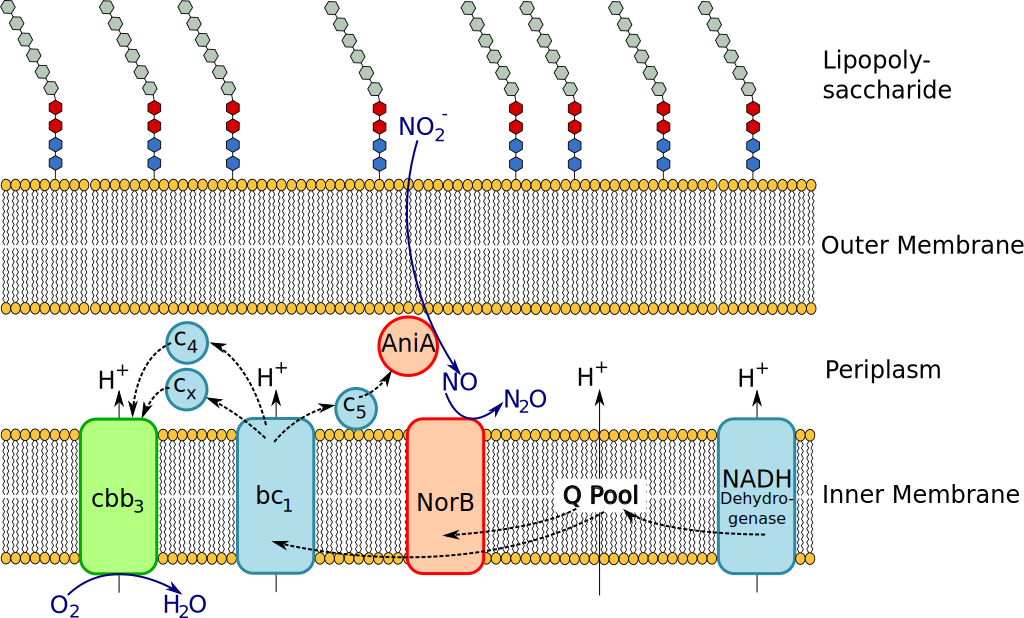
\includegraphics[width=14cm]{./01-introduction/data/Respiratory_layout.pdf}
 % Respiratory_layout.pdf: 819x404 pixel, 72dpi, 28.89x14.25 cm, bb=0 0 819 404
\end{center}
\caption{\footnotesize {\bf Layout of the components of the respiratory system in \Nsm{}.} Oxygen reducing components are shown in green, nitrogen reducing components in red. Components transporting electrons are coloured light blue, and their transport is indicated by dashed arrows. Respiratory substrates are shown in dark blue, with corresponding arrows linking them to their reducing enzymes. Components which produce membrane potential are also indicated.
\label{fig:etc}}
\end{figure}

In addition to the difference in favourability between the two respiratory pathways, there is also a great deal of regulation, both at the enzymatic and transcriptional level. Chemical inhibition also plays a part in regulation as briefly mentioned previously. Expression of AniA is regulated by two processes, the reduction of oxygen and the presence of nitrite. The presence of oxygen down-regulates the expression of an activator of AniA expression. This activator is FNR (fumarate and nitrate reduction regulator)\nomenclature{FNR}{Fumarate and Nitrite reduction Regulator}, and the presence of oxygen effectively means that AniA expression is repressed by the reduced expression of FNR. In \Nm{}, FNR appears to work slightly differently than in facultative anaerobes such as \textit{E. coli}, in that FNR is still expressed at quite high concentrations of oxygen, and is itself down-regulated by a separate co-factor \cite{Rock2007}.

The presence of nitrite triggers the two component NarP/NarQ\nomenclature{NarP}{Nitrate/Nitrite Response Regulator}\nomenclature{NarQ}{Nitrate/Nitrite Response Sensor} system which activates expression of AniA in response to increasing levels of nitrite \cite{Rock2005}. The activity of AniA is also controlled by the competition for electrons by the other reductase enzymes in the respiratory chain. Both NorB and \cbbthree{} have a higher affinity for electrons than AniA, and as a result the presence of these enzymes (when active) has an inhibitory effect on AniA. The regulation of AniA is further complicated by the production of nitric oxide, and the presence of a protein, NsrR\nomenclature{NsrR}{Nitrite sensing repressor protein}.

Nitric oxide has a direct inhibitory effect on the expression of AniA, as does the NsrR protein. Nitric oxide also inhibits the NsrR protein, leading to a de-represssion of AniA \cite{Heurlier2008}. In the absence of nitric oxide, AniA is almost fully repressed by active NsrR. As \cNO{} concentrations increase, NsrR is inactivated allowing full activation of AniA. Once \cNO{} reaches a sufficiently high level it will begin to inhibit AniA \cite{Rock2005,Rock2007}.

NorB is less tightly regulated by respiratory components, as it is only acted upon by NsrR, however it is regulated by FNR and ArsR outside the respiratory chain \cite{VincentIsabella01012008}. This regulation by NsrR works in a similar way to how NsrR acts upon AniA. When there is no nitric oxide present, the NsrR acts to inhibit NorB since there is no substrate for it to reduce. In the presence of nitric oxide, NsrR is inhibited, leading to the activation of NorB which is now able to reduce \cNO{} to \cNtwoO{}. In this case nitric oxide is acting as a de-repressor of NorB.

This complicated set of regulatory relationships between the different components of the respiratory pathways is shown in Figure \ref{fig:respiratory-pathway}.

\begin{figure}
 \begin{center}
 \includegraphics[width=14cm]{./01-introduction/data/regulation.pdf}
\end{center}
\caption{\footnotesize {\bf Regulation of respiratory components in \Nsm{}.} Enzymes and enzymatic reactions are shown in red. \textit{A.} describes the regulation caused by competetion for electrons between the respiratory enzymes. \textit{B.} shows the genetic regulation, which also involves a number of additional components in dark blue. \textit{C.} shows chemical inhibition of the respiratory components.
\label{fig:respiratory-pathway}}
\end{figure}

\section{Modelling}

A limited amount of modelling has been carried out on bacterial respiratory chains, these focused on the denitrification pathway and treated the pathway as a simple electrical circuit \cite{almeida_unifying_1997}. An alternative approach involved modeling respiration using ``P systems'' which are probabilistic models of events. This assigned a probability of each reaction happening, dependant on the state of the system and then iterated through a given set of steps evaluating probabilities and altering values based on the outcome \cite{cavaliere_modeling_2006}. This approach to modelling was limited in that it was only predicting the quantities of 1 component in each of 2 ``compartments''; oxygen in the cell membrane and carbon dioxide in the thylakoid membrane (the model was developed using cyanobacteria).

Since when modelling respiration in a cell, the most important factor is the change in concentration of components over time without any particular spatial constraints, ordinary differential equations (ODEs)\nomenclature{ODE}{Ordinary Differential Equation} are an appropriate technique. In these systems the model does not change with regard to the spatial arrangement of any of the components. If the system requires changes in time \textit{and} space, then partial differential equations (PDEs)\nomenclature{PDE}{Partial Differential Equation} would be necessary (and more complicated) \cite{Klipp2005}.

Ordinary differential equations only depend on one variable; the time ($t$). In this case, the change in concentration over time for each component can be modelled as a single differential equation. For multiple components this leads to multiple differential equations with some that rely on the result of another (if the rate of one reaction is directly related to the concentration of another component). These ODEs must then be solved in parallel at a suitable timescale.

Complications arise when using differential equations if the processes are considered to be stochastic, as a differential equation model assumes that every component can have a continuous value, which is not the case as molecules are discrete. However if the system being modeled is sufficiently large, this effect can be ignored. If the reaction component size is small ($<$ 100s of molecules) stochastic simulation algorithms have to be used as described by \citet{Gillespie1977}. This method requires far more computation than solving ODEs, as the model will spend most of its time calculating values for reactions involving large molecules even though this is not necessary as the reaction is not stochastic. Additionally, the time interval used between reaction steps is usually very small, meaning the simulation progresses slowly \cite{Klipp2005}.

A number of software packages exist that are capable of this type of modeling such as the Systems Biology Workbench \cite{Sauro2003} and COPASI \cite{StefanHoops12152006}. These allow you to enter biochemical reactions in a format familiar to biologists, and have pre-defined libraries for types of reactions such as mass-action, or one with Michaelas-Menton kinetics etc. The mathematical equations are then derived automatically from the reactions and can be modified by hand if necessary. Parameters for the mathematical equations must be entered, and these will usually be derived from experimental data, or in some cases educated guesses (at least initially). Once a parameter set has been created, the modelling software can run a time-course using a relevant solver-algorithm. COPASI includes 4 solvers,  LSODA (Livermore Solver for Ordinary Differential Equations) \cite{RH93} for deterministic systems (such as ODEs), Gibson-Bruck \cite{Gibson2000} for stochastic systems and Runge-Kutta and LSODA for hybrid systems (where portions are not considered to be stochastic).

\chapter{Materials and Methods}
\section{\Nsm\space strains used in this work}
\begin{table}[here]
\begin{center}
\begin{tabular}{|c|p{7cm}|c|}
\hline
\textbf{Name} & \textbf{Description} & \textbf{Source} \\
\hline
MC58 & Wild-Type Strain & Mel, via Karin \\
&&\\ %cheat for extra whitespace beneath each entry
\hline
$\Delta$norB::spc$^\textrm{r}$ & Wild-Type with insertion of spectinomycin resistance cassette into \textit{norB} gene & \citet{Heurlier2008} \\
&&\\ %cheat for extra whitespace beneath each entry
\hline
$\Delta$nsrR::spc$^\textrm{r}$ & Wild-Type with insertion of spectinomycin resistance cassette into \textit{nsrR} gene & \citet{Rock2007} \\
&&\\ %cheat for extra whitespace beneath each entry
\hline
$\Delta$norB::spc$^\textrm{r}$-$\Delta$nsrR::tet$^\textrm{r}$ & Wild-Type with insertion of spectinomycin resistance cassette into \textit{norB} and insertion of tetracyclin resistance cassette into \textit{nsrR} genes & \citet{Heurlier2008}\\
&&\\ %cheat for extra whitespace beneath each entry
\hline
$\Delta$aniA::spc$^\textrm{r}$-$\Delta$nsrR::tet$^\textrm{r}$ & Wild-Type with insertion of spectinomycin resistance cassette into \textit{aniA} and insertion of tetracyclin resistance cassette into \textit{nsrR} genes & \citet{Heurlier2008} \\
&&\\ %cheat for extra whitespace beneath each entry
\hline
\end{tabular} 
\end{center}
\small{\caption{Bacterial strains and sources}
\label{tab:bacterial-strains}}
\end{table}

\section{Culturing \Nsm}
\subsection{Growth of \Nsm}
\Nm\space strains were grown on plates on Columbia Agar Base with defibrinated horse blood, and in liquid culture in Muller-Hinton Broth (MHB)

Plates were prepared by adding horse blood to a final concentration of 5\% to molten agar, and poured into plastic petri dishes. After streaking with \Nm\space the plates were incubated at 37\textdegree C in a 5\% carbon dioxide/air mixture.

Aerobic liquid cultures were grown in 10ml MHB with 1\% NaHCO$_\textrm{3}$ in plastic sterilin tubes, and incubated at 37\textdegree C at 200rpm. Microaerobic cultures were suspended in 20ml MHB, 1\% NaHCO$_\textrm{3}$ in plastic sterilin tubes, incubated at 37\textdegree C at 100rpm.

\subsection{Preparation of Antibiotic Selective Media}
Liquid stock solutions of required antibiotics were either added directly to liquid culture, or, if growing on plates, to the molten agar when also adding horse blood. The final concentrations of antibiotics are given in Table \ref{tab:antibiotic-concs}.

\begin{table}[here]
\begin{center}
\begin{tabular}{c|c}
\textbf{Antibiotic} & \textbf{Final concentration ($\mu$g/ml)} \\
\hline
Spectinomycin & 50 \\
Tetracyclin & 2.5 \\
Chloramphenicol & 50 \\
\hline
\end{tabular} 
\end{center}
\small{\caption{Final antibiotic concentrations}
\label{tab:antibiotic-concs}}
\end{table}

\subsection{Preparation of Frozen Bacterial Stocks}
Bacteria were grown in liquid culture until late log phase prior to harvesting. Liquid cultures were then centrifuged at 4000g for 15 minutes, and the pellet was then resuspended in a 25\% glycerol, 25\% water and 50\% MHB, all of which had been autoclaved beforehand. The bacterial stocks were then frozen at $-80$\textdegree C.

\subsection{Streaking Plates for OD to CFU Ratio Calculation}
Bacterial cultures were grown overnight and then transferred into aerobic liquid culture and samples taken throughout the day to obtain a range of different optical densities. The optical density was recorded at 600nm, and each sample was serially diluted to the following levels: $10^{-5}$, $10^{-6}$ and $10^{-7}$. 100$\mu$l of each of these dilutions was plated on a fresh blood agar plate and left to grow overnight. The following morning the number of colonies on each plate was counted and used to create a standard curve for Optical Density to Colony Forming Units.

\section{Measuring Oxygen Concentration}
Oxygen concentration in respiring cultures was measured using a Clark electrode \cite{Clark1953} from Rank Brothers, Cambridge, UK. This electrode has a silver anode and a platinum cathode using a saturated potassium chloride solution as electrolyte. The electrode is set at the bottom of a ~7ml reaction chamber separated from its contents by a thin teflon membrane. This membrane is permeable to dissolved oxygen, and is reduced by the electrode producing a measurable electrical current. The reaction chamber is maintained at 37\textdegree C by an attached waterbath.
When performing experiments, 5ml of culture is added to the reaction chamber, which is stirred by use of a magnetic flea, and the chamber covered with a plastic stopper. The stopper has a number of holes through which the NO probe, or hamilton syringe can be inserted. Data is collected by attaching the electrode to an external data logger (Pico ADC20, Pico Technology).
\subsection{Calibration of Oxygen Electrode}
Calibration of the oxygen electrode assumes that anaerobic water will not produce any measurable current at the electrode. Oxygen saturated water contains 210$\mu$M Oxygen (ref needed). 5ml of ultrapure water was added to the electrode chamber, and then aerated to saturation by use of a pasteur pipette. The maximum value recorded by the data logger then corresponds to a concentration of 210$\mu$M Oxygen, with the relationship between mV as recorded against concentration being linear.

\section{Measuring Nitric Oxide Concentration}
Nitric Oxide concentration was measured using a Nitric Oxide probe (ISO-NOP, World Precision Intruments) connected to a Nitric Oxide Meter (ISO-NO mkII, World Precision Instruments). The NO probe is inserted through one of the holes in the plastic lid of the reaction chamber of the oxygen electrode assembly. The tip of the electrode should be immersed in the culture, with care being taken not to trap any air bubbles on the surface of the probe. The sensor is also attached to the same data logger as above. In this way both Oxygen and Nitric Oxide concentrations can be measured in parallel.
\subsection{Calibration of Nitric Oxide Electrode}
Calibration of the nitric oxide electrode 

\section{Measuring Nitrite Concentration (Griess Assay)}
\cite{DonaldNicholas1957}
\subsection*{Chemicals}
\begin{itemize}
 \item 50ml 1\% w/v Sulfanilamide in 1M HCl
 \item 50ml 0.02\% w/v N.E.D. in 1M HCl
\end{itemize}


\section{Nitric Oxide Production}
\begin{figure}
 \centering
 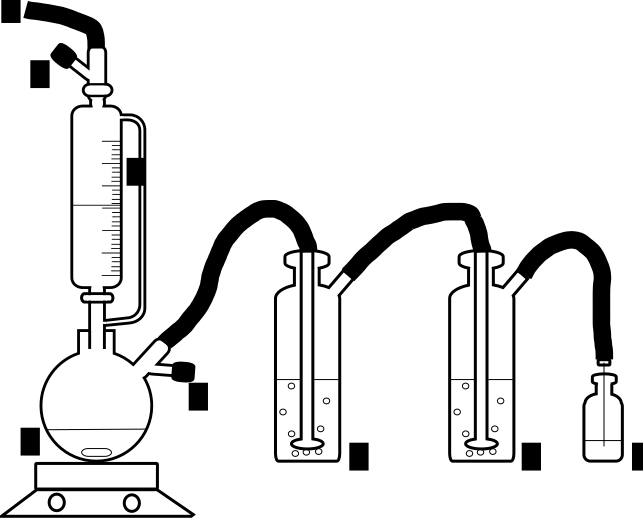
\includegraphics[width=14cm]{./02-materialsmethods/data/drawing.pdf}
 % drawing.pdf: 515x415 pixel, 72dpi, 18.17x14.64 cm, bb=0 0 515 415
 \caption{\footnotesize NO making apparatus. 1,2 - N$_{\textrm{2}}$ release valve. 3 - 50ml 4M H$_{\textrm{2}}$SO$_{\textrm{4}}$. 4 - 200ml 2M NaNO$_{\textrm{2}}$ stirring. 5 - 1M NaOH $\frac{2}{3}$ full. 6,7 - dH$_{\textrm{2}}$O $\frac{2}{3}$ full. 8 - To N$_{\textrm{2}}$ gas bottle.}
\end{figure}
\subsection*{Chemicals}
\begin{itemize}
 \item 200ml NaNO$_{\textrm{2}}$ @ 2M - 27.6g in 200ml dH$_{\textrm{2}}$O
 \item 50ml H$_{\textrm{2}}$SO$_{\textrm{4}}$ @ 4M - 11ml in 39ml dH$_{\textrm{2}}$O
 \item 200ml NaOH @ 1M - 8g in 200ml dH$_{\textrm{2}}$O
\end{itemize}

\subsection*{Procedure}
\begin{itemize}
 \item Set up system and sparge with N$_{\textrm{2}}$ gas for 15 minutes. Sparge 4M H$_{\textrm{2}}$SO$_{\textrm{4}}$ separately.
 \item Shut valve to N$_{\textrm{2}}$ hose (blue valve 1).
 \item Keep blue valve 2 open at all times.
 \item When sparged, add 25ml of 4M H$_{\textrm{2}}$SO$_{\textrm{4}}$ to 2M NaNO$_{\textrm{2}}$ and allow brown gas to bubble through to saturated solution vessel.
 \item Leave for at least 15 minutes allow 2M solution to cool.
 \item Remove needle and close sealing valve on saturated solution vessel.
 \item Clean up - allow 1-2 hours to allow reaction to finish. Sparge with N$_{\textrm{2}}$ to get rid of residual NO gas. Disassemble, wash in dH$_{\textrm{2}}$O and dry in oven.
\end{itemize}

\chapter{Model - Construction and Parameters}
\section{Construction}
\subsection{Converting Biological Reactions into Differential Equations}
Where the reaction is describing a chemical process, the rate constant is given above the arrow, and the relevant enzyme shown in parentheses. Where the reaction is showing the addition of electrons (reduction), this is denoted by $e^-$ below the arrow, the rate constant above, and the source of electrons in parentheses.

The equation that gives the change in oxygen concentration is

\begin{eqnarray}
&\frac{d[O_2]}{dt} = \beta(1-[O_2]/K_O) - k_{1}[C_a][O_2] \nonumber \\\nonumber \\
&\xrightarrow{\beta} \mathbf{O_2} \xrightarrow{k_1~(C_a)} \textnormal{H$_\textnormal{2}$O}
\label{eq:oxygen}
\end{eqnarray}

where $\beta$ is the rate of passive diffusion of \cOxygen \space into the electrode chamber. This is inversely proportional to oxygen concentration in the chamber, and limited to the oxygen saturation concentration, $K_O$. This component of the equation is required to account for a peculiarity of the experimental set-up, whereby the rate of diffusion of oxygen into the system depends on the density of the bacterial culture, and is not insignificant. $k_{1}$ is the rate of reduction of oxygen by the oxygen reductase \textit{cbb$_{\textrm{3}}$}. This rate depends on the concentration of reduced (i.e. active) \textit{cbb$_{\textrm{3}}$}, $C_a$ and the concentration of \cOxygen.

The equation for describing \cNO \space concentration changes is more complex as \cNO \space has a number of additional interactions in comparison to \cOxygen. \cNO \space also interacts with \textit{cbb$_{\textrm{3}}$}, in addition to being reduced from \cNitrite, reduced to \cNtwoO \space and spontaneously lost from the electrode chamber. Currently this is the equation being used to model \cNO \space concentration.

\begin{eqnarray}
&\frac{d[NO]}{dt} = m_{1}[NO_2^-][A_a] - l_1[NO][B_a] - k_5[C_a][NO] + k_6 [C_X] - \gamma[NO] \nonumber \\\nonumber \\
&\textnormal{NO$_\textnormal{2}^\textnormal{-}$} \xrightarrow{m_1~(A_a)} \mathbf{NO} \xrightarrow{l_1~(B_a)} \textnormal{N$_\textnormal{2}$O} \nonumber \\
&\mathbf{NO} + \textnormal{C$_\textnormal{a}$} \xrightarrow{k_5} \textnormal{NO}\textendash \textnormal{C$_\textnormal{X}$} \xrightarrow{k_6} \mathbf{NO} + \textnormal{C$_\textnormal{a}$} \nonumber \\
&\xrightarrow{\gamma} \mathbf{NO}
\label{eq:no}
\end{eqnarray}

The synthesis of \cNO \space is modelled by $m_{1}$ which is the rate of \cNitrite \space reduction by reduced (active) AniA. This also depends on the concentration of \cNitrite \space and reduced AniA ($A_a$). The reduction of \cNO \space requires $l_1$ which is the rate of reduction of \cNO \space by reduced (active) NorB. This depends on the concentration of \cNO \space and reduced NorB ($B_a$). Inhibition of \textit{cbb$_{\textrm{3}}$} by \cNO \space is modelled by the \engordnumber{3} component of the equation. $k_5$ is the rate of inhibition of \textit{cbb$_{\textrm{3}}$} by \cNO. $k_6$ is the rate of recovery of inhibited \textit{cbb$_{\textrm{3}}$}. $\gamma$ is the rate of spontaneous loss of \cNO \space from the electrode chamber.

The reduction of nitrite is modelled by this equation

\begin{eqnarray}
&\frac{d[NO_2^-]}{dt} = - m_{1}[NO_2^-][A_a] \nonumber \\\nonumber \\
&\mathbf{NO_2^-} \xrightarrow{m_1~(A_a)} \textnormal{NO}
\label{eq:nitrite}
\end{eqnarray}

where $m_{1}$ is the rate of reduction of \cNitrite by reduced (active) AniA ($A_a$).

In addition to the rate of change of concentration of the respiratory substrates, the model also contains information about the state of the quinone pool, which is the upstream source of electrons into the respiratory chain. This is important because this affects the rate of reduction of the various enzymes which perform the substrate reductions. The equation for modelling the change in reduction state (activity) of the quinone pool is

\begin{eqnarray}
&\frac{d[Q_a]}{dt} = g([Q] - [Q_a]) - l_3[Q_a]([B] - [B_a]) - f[Q_a]([X]-[E]) \nonumber \\\nonumber \\
&\xrightarrow[e^-]{g} \mathbf{Q_a} \nonumber \\
&\textnormal{B$_\textnormal{i}$} \xrightarrow[e^-]{l_3~(\mathbf{Q_a})} \textnormal{B$_\textnormal{a}$} \nonumber \\
&\textnormal{X-E} \xrightarrow[e^-]{f~(\mathbf{Q_a})} \textnormal{E}
\label{eq:quinones}
\end{eqnarray}

$Q_a$ is the reduced quinone, and $Q$ the total concentration of quinones in the system. $g$ represents the rate of flow of electrons into the quinone pool from NADH. The rate of reduction of NorB by active quinones is given by $l_3$. NorB and reduced NorB are given by $B$ and $B_a$ respectively. As the quinones also reduce the cytochromes, this also needs to be modelled. $f$ denotes the rate of reduction of cytochromes by the active quinones. Cytochromes and reduced cytochromes are given by $X$ and $E$ respectively.

Given that the concentration of active cytochromes changes, due to reduction by the quinone pool and oxidation by the downstream enzymes, and this concentration is a parameter in (\ref{eq:quinones}), it also needs to be included in the model, and this is given by the following equation

\begin{eqnarray}
&\frac{d[E]}{dt} = -k_3([C] - [C_a] - [C_X])[E]  - m_3([A] - [A_a])[E] + f[Q_a]([X]-[E]) \nonumber \\\nonumber \\
&\textnormal{C$_\textnormal{i}$} \xrightarrow[e^-]{k_3~(\mathbf{E})} \textnormal{C$_\textnormal{a}$} \nonumber \\
&\textnormal{A$_\textnormal{i}$} \xrightarrow[e^-]{m_3~(\mathbf{E})} \textnormal{A$_\textnormal{a}$} \nonumber \\
&\textnormal{X-E} \xrightarrow[e^-]{f~(Q_a)} \mathbf{E}
\label{eq:cytochromes}
\end{eqnarray}

where $k_3$ is the rate of reduction of the cytochrome c oxygen reductase (\textit{cbb$_{\textrm{3}}$}) by the quinone pool (via \textit{c$_{\textrm{x}}$} \& \textit{c$_{\textrm{4}}$}). $C$, $C_a$ and $C_X$ represent the overall concentration of \textit{cbb$_{\textrm{3}}$}, reduced (active) \textit{cbb$_{\textrm{3}}$} and denatured \textit{cbb$_{\textrm{3}}$} respectively. $m_3$ is the rate of reduction of AniA by the cytochrome pool (via \textit{c$_{\textrm{5}}$}). The concentration of active cytochromes increases by their reduction by the quinone pool.

To model the changes in concentration of the individual enzymes, \textit{cbb$_{\textrm{3}}$}, AniA and NorB, the following equations are used:

\begin{eqnarray}
&\frac{d[C_a]}{dt} = k_3([C] - [C_a] - [C_X])[E] - k_{1}[C_a][O_2] - k_5[C_a][NO] \nonumber \\\nonumber \\
&\textnormal{C$_\textnormal{i}$} \xrightarrow[e^-]{k_3~(E)} \mathbf{C_a} \nonumber \\
&\textnormal{O$_\textnormal{2}$} \xrightarrow{k_1~(\mathbf{C_a})} \textnormal{H$_\textnormal{2}$O} \nonumber \\
&\textnormal{NO} + \mathbf{C_a} \xrightarrow{k_5} \textnormal{NO}\textendash \textnormal{C$_\textnormal{X}$}
\label{eq:active_cbb3}
\end{eqnarray}

This equation models the concentration of reduced (active) \textit{cbb$_{\textrm{3}}$}, and the following equation models the concentration of \textit{cbb$_{\textrm{3}}$} that has been denatured by \cNO.

\begin{eqnarray}
&\frac{d[C_X]}{dt} = k_5[C_a][NO] - k_6 [C_X] \nonumber \\\nonumber \\
&\textnormal{NO} + \textnormal{C$_\textnormal{a}$} \xrightarrow{k_5} \textnormal{NO}\textendash \mathbf{C_X} \xrightarrow{k_6} \textnormal{NO} + \textnormal{C$_\textnormal{a}$}
\label{eq:denatured_cbb3}
\end{eqnarray}

Reduced (active) AniA concentrations are modelled by this equation

\begin{eqnarray}
&\frac{d[A_a]}{dt} = m_3([A] - [A_a])[E]- m_{1}[NO_2^-][A_a] \nonumber \\\nonumber \\
&\textnormal{A$_\textnormal{i}$} \xrightarrow[e^-]{m_3~(E)} \mathbf{A_a} \nonumber \\
&\textnormal{NO$_\textnormal{2}^\textnormal{-}$} \xrightarrow{m_1~(\mathbf{A_a})} \textnormal{NO}
\label{eq:active_ania}
\end{eqnarray}

and reduced (active) NorB concentrations are modelled by this equation

\begin{eqnarray}
&\frac{d[B_a]}{dt} = l_3[Q_a]([B] - [B_a]) - l_1[NO][B_a] \nonumber \\\nonumber \\
&\textnormal{B$_\textnormal{i}$} \xrightarrow[e^-]{l_3~(Q_a)} \mathbf{B_a} \nonumber \\
&\textnormal{NO} \xrightarrow{l_1~(\mathbf{B_a})} \textnormal{N$_\textnormal{2}$O}
\label{eq:active_norb}
\end{eqnarray}

\subsection{Assumptions and their Justifications}
\section{Parameters}
\chapter{Parameter Estimation Methodologies}
\section{Simulated Annealing}
\section{Approximate Bayesian Computation by Sequential Monte Carlo}
\section{Metropolis Hastings Monte Carlo}
\chapter{Oxygen Reduction in \Nm{}}
\section{Aerobic Reduction of Oxygen}
\subsection{Introduction}
\subsection{Results}
\subsection{Discussion}
\svnid{$Id$}
\chapter{Nitric Oxide Reduction in \Nm{}}
\label{chap:noreduction}
\section{Aerobic Nitric Oxide Reduction}
\subsection{Introduction}
The next dataset used in the iterative approach to parameter estimation was of aerobic oxygen reduction interrupted by the addition of Nitric Oxide. These datasets are the next most complicated after aerobic oxygen reduction as it introduces the nitric oxide reduction pathway. In this case the oxygen reduction and Nitric Oxide reduction pathways are active. Additionally, inactivation of \cbbthree{} by Nitric Oxide was occurring. The portions of the ETC relating to Nitric Oxide reduction are shown graphically in Figure \ref{fig:no_resp_chain}. However this pathway cannot be isolated \textit{in vivo} as \Nm{} is incapable of completely anaerobic respiration therefore the required parts of the model are actually those from Chapter \ref{chap:oxygenreduction} and those in Figure \ref{fig:no_resp_chain}.
\begin{figure}[tbp]
  \centering
    \includegraphics[width=14cm]{06-noreduction/data/no_resp_chain.pdf}
    \caption[Nitric oxide reducing electron transport chain of \Nm{}]{{\bf Nitric oxide reducing electron transport chain of \Nm{}.} This shows the complete electron transport chain of \Nsm{} with the components irrelevant to nitric oxide reduction greyed out.
  \label{fig:no_resp_chain}}
\end{figure}\\
The equations that describe this portion of the ETC are:
\begin{eqnarray*}
\frac{d[O_2]}{dt} & = & \beta(1-[O_2]/K_O) - k_{1}[C_a][O_2]\\
\frac{d[Q_a]}{dt} & = & g([Q] - [Q_a]) - l_3[Q_a]([B] - [B_a]) - f[Q_a]([X]-[X_a])\\
\frac{d[X_a]}{dt} & = & -k_3([C] - [C_a] - [C_X])[X_a]  - m_3([A] - [A_a])[X_a] + f[Q_a]([X]-[X_a])\\
\frac{d[C_a]}{dt} & = & k_3([C] - [C_a] - [C_X])[X_a] - k_{1}[C_a][O_2] - k_5[C_a][NO] + k_6[C_X]\\
\frac{d[NO]}{dt} & = & m_{1}[NO_2^-][A_a] - l_1[NO][B_a] - k_5[C_a][NO] + k_6 [C_X] - \gamma[NO]\\
\frac{d[C_X]}{dt} & = & k_5[C_a][NO] - k_6 [C_X]\\
\frac{d[B_a]}{dt} & = & l_3[Q_a]([B] - [B_a]) - l_1[NO][B_a]
\end{eqnarray*}
These equations describe the change in concentration of Nitric Oxide over time, which is the experimentally observable value (in addition to the afore modelled oxygen). Also being modelled was the change in concentration of inhibited \cbbthree{} and the reduction state of NorB. This more complete portion of the model involved 24 parameters and variables which were to be estimated. This number includes the 13 values already estimated in Chapter \ref{chap:oxygenreduction}.
\subsection{Experimental Results}
Generation of Nitric Oxide reduction datasets required the growth of MC58 (wild type \Nsm{}) in aerobic conditions until mid log-phase growth had been achieved. This corresponds to an $OD_{600}$ of 0.3-0.9 and usually required an incubation period of roughly 3 hours. Once the required cell density had been obtained, the culture was transferred to the oxygen electrode chamber and the oxygen and nitric oxide concentrations recorded as the culture respired. To model nitric oxide reduction required that nitric oxide solution was added to the culture while it is respiring aerobically. Part-way through aerobic respiration nitric oxide solution was added to various final concentrations all at $\approx 5~\mu$M and the culture then left to reduce nitric oxide (in addition to oxygen). The nitric oxide reduction datasets generated and used for parametrisation of this portion of the model are shown in Figures \ref{fig:nodata}, \ref{fig:nodata2}, \ref{fig:nodata1} \& \ref{fig:nodata3}. Unfortunately the experimental data upon addition of nitric oxide is very difficult to reliably reproduce, with different cultures having apparently different tolerances to nitric oxide (data not shown).

%ds1
\begin{figure}[tbp]
 \centering
 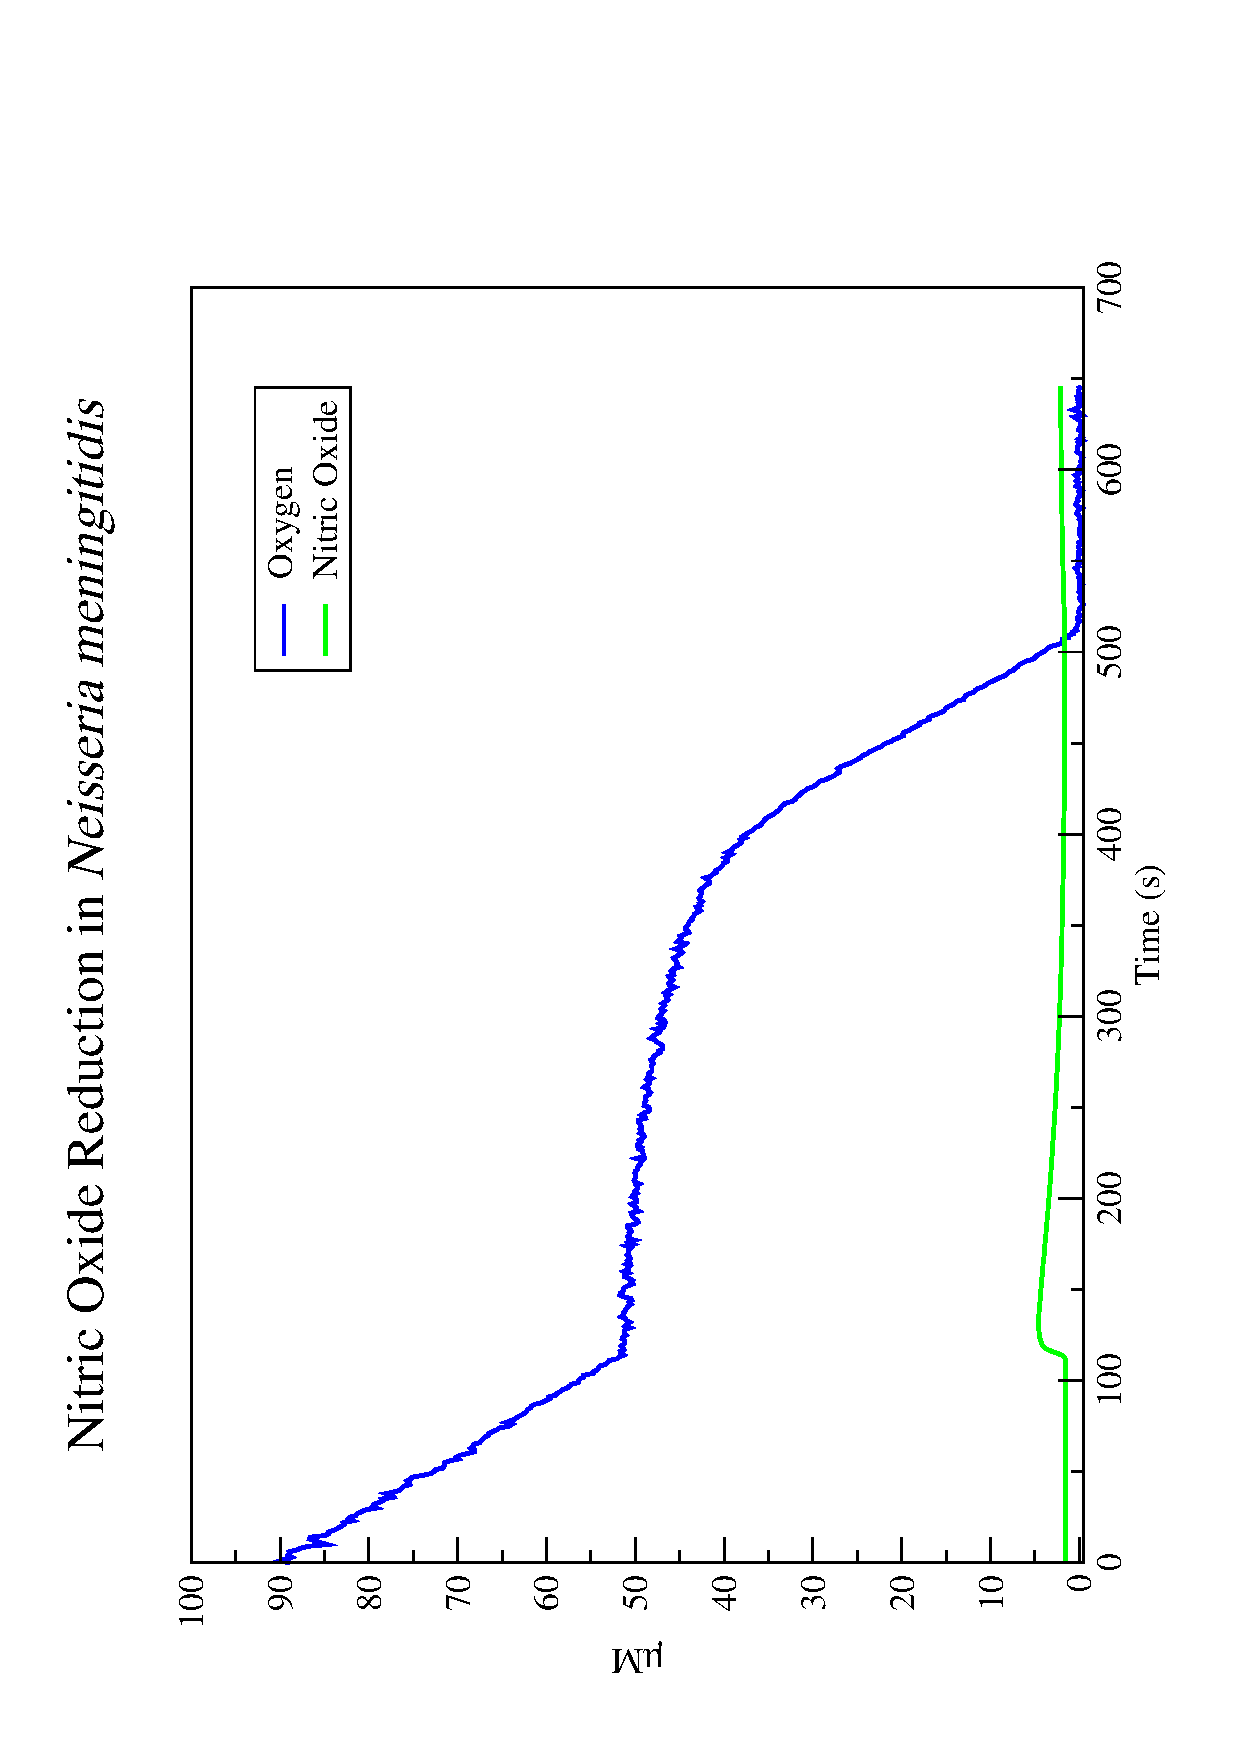
\includegraphics[height=10cm, trim=1cm 1cm 3cm 1cm, clip=true]{./06-noreduction/data/aer-no-data.pdf}
 % nosim.eps: 0x0 pixel, 300dpi, 0.00x0.00 cm, bb=0 0 794 595
 \caption[{Nitric Oxide Reduction in \textit{Neisseria meningitidis}.}]{{\bf Nitric Oxide Reduction in \textit{Neisseria meningitidis}.} This dataset shows the effect on rate of oxygen reduction as nitric oxide (to $\approx 3~\mu M$) is introduced to the respiring system which also appears to have been partially primed for nitric oxide reduction. Note that the increase in nitric oxide concentration seen at the end of the dataset is most likely due to drift in the electrode.}
 \label{fig:nodata}
\end{figure}
The dataset in Figure \ref{fig:nodata} appears to show a system that was partially primed for microaerobic respiration. In this case it was speculated that there was a small amount of NorB (nitric oxide reductase) present. Initially the oxygen reduction was carried out in exactly the same manner as in Chapter \ref{chap:oxygenreduction}. Upon addition of nitric oxide, oxygen respiration slowed and almost stopped as a result of competition for electrons between \cbbthree{} and NorB, and the direct chemical inhibition of \cbbthree{} by NO. Nitric oxide started to be removed as a combination of diffusion (although this rate will be low as shown in the previous two datasets) and reduction via NorB. Once the NO has been removed from the system oxygen reduction resumes at almost the same rate as before and still has the same high affinity feature as the oxygen reduction datasets in Chapter \ref{chap:oxygenreduction}.

%ds2
\begin{figure}[tbp]
 \centering
 \includegraphics[height=10cm, trim=1cm 1cm 3cm 1cm, clip=true]{./06-noreduction/data/aer-no-data2.pdf}
 % nosim.eps: 0x0 pixel, 300dpi, 0.00x0.00 cm, bb=0 0 794 595
 \caption[{Nitric Oxide Reduction in \textit{Neisseria meningitidis}.}]{{\bf Nitric Oxide Reduction in \textit{Neisseria meningitidis}.} This dataset shows the effect on rate of oxygen reduction as a larger amount of nitric oxide (to $\approx 7.8~\mu M$) is introduced to the respiring system.}
 \label{fig:nodata2}
\end{figure}
The dataset in Figure \ref{fig:nodata2} shows a larger change in the rate of oxygen reduction than that of Figure \ref{fig:nodata1} when a larger amount of nitric oxide is introduced. Again the removal of nitric oxide will primarily be due to diffusion, although now at higher concentrations more nitric oxide will interact with \cbbthree{} temporarily inhibiting it. This inhibition causes the reduction in oxidase activity, and the sequestering of NO by \cbbthree{} also causes some of the visible reduction in nitric oxide concentration. The time-scale over which the nitric oxide disappears strongly suggests that it is not due to nitric oxide reductase activity. It may also be possible that at this concentration of nitric oxide some \cbbthree{} may have been permanently inhibited as mentioned in Chapters \ref{chap:intro} \& \ref{chap:model}. As the cultures in this dataset were obviously being negatively affected by the addition of such a high concentration of nitric oxide, either by permanent inhibition of \cbbthree{} or actual cell death, it was unlikely that this particular dataset could be used to accurately predict parameters in the model as it includes factors that were never part of the original model.

%ds3
\begin{figure}[tbp]
 \centering
 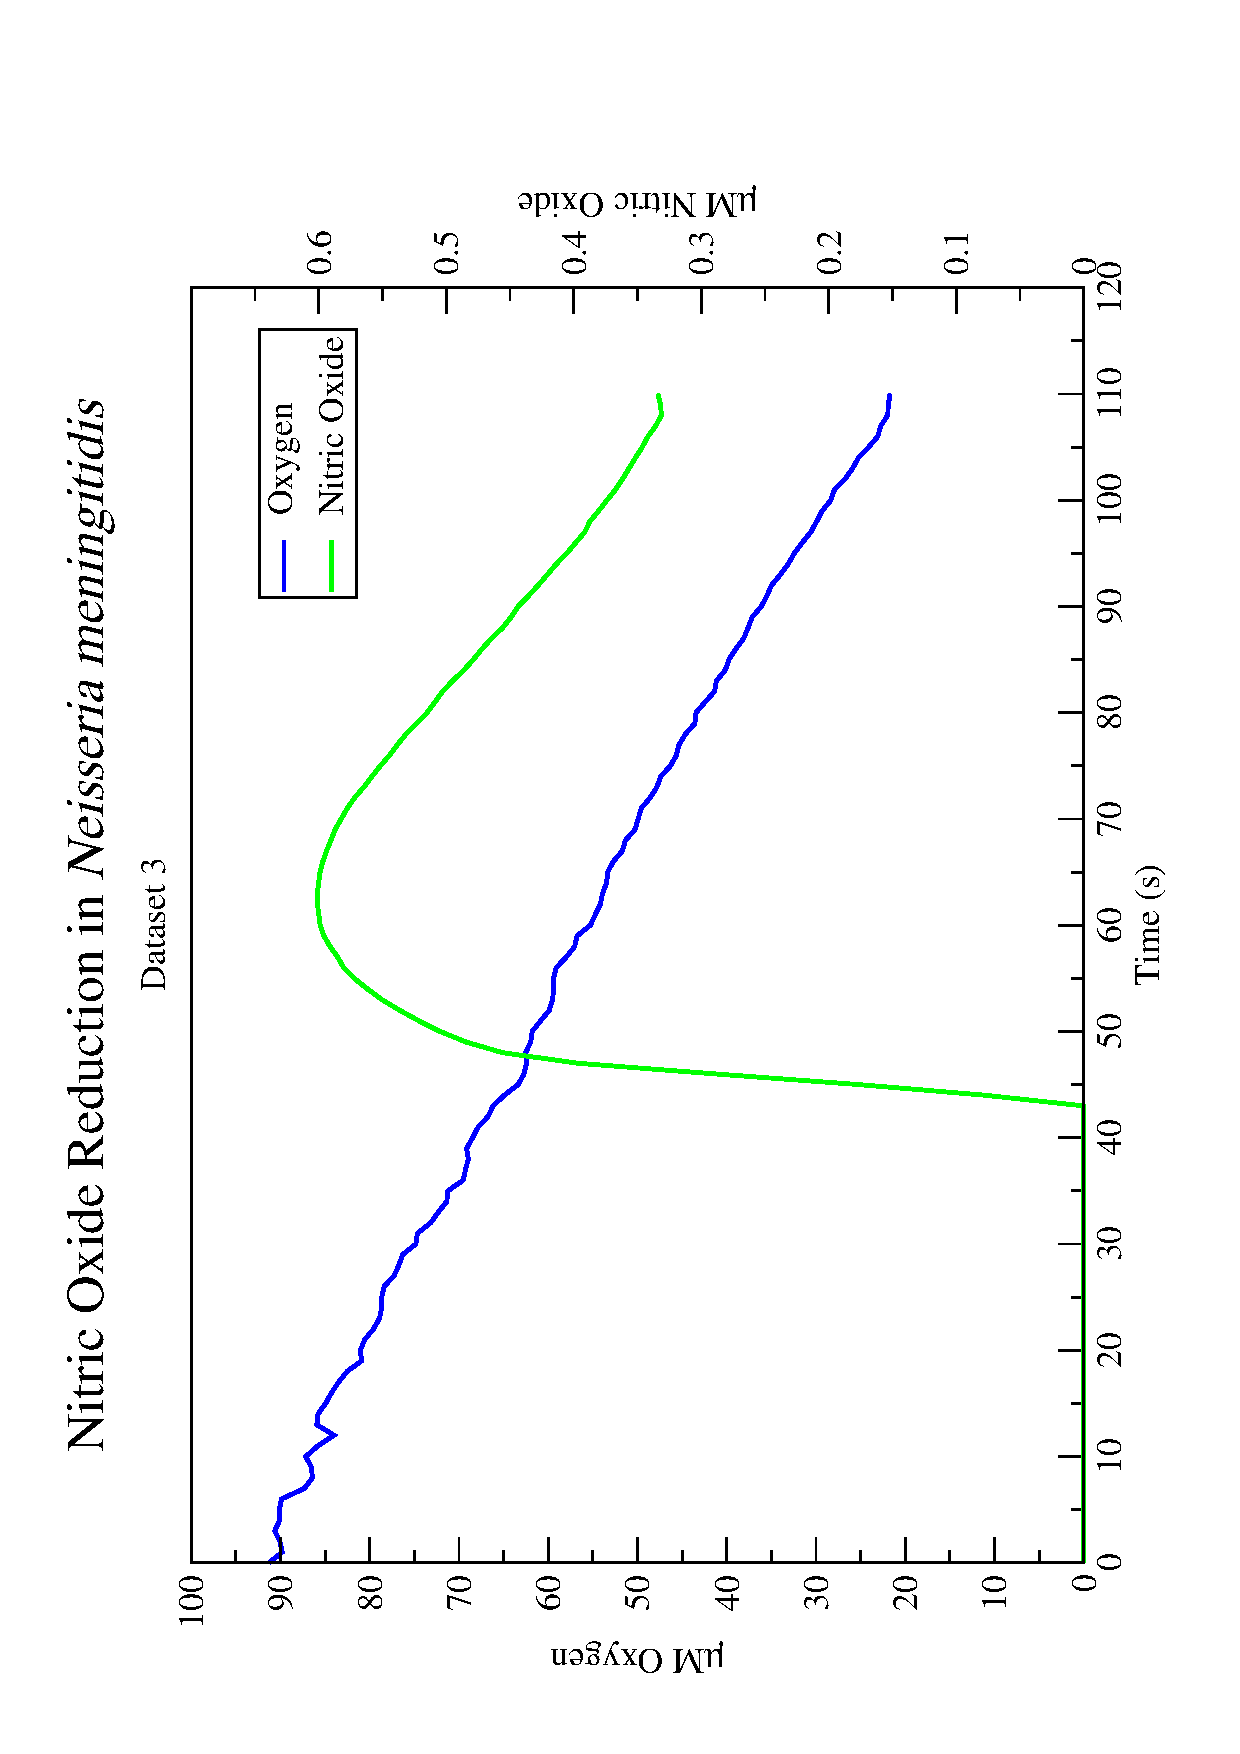
\includegraphics[height=10cm, trim=1cm 1cm 3cm 1cm, clip=true]{./06-noreduction/data/aer-no-data1.pdf}
 % nosim.eps: 0x0 pixel, 300dpi, 0.00x0.00 cm, bb=0 0 794 595
 \caption[{Nitric Oxide Reduction in \textit{Neisseria meningitidis}.}]{{\bf Nitric Oxide Reduction in \textit{Neisseria meningitidis}.} This dataset shows the effect on rate of oxygen reduction as a small amount of nitric oxide (to $\approx 0.6~\mu M$) is introduced to the respiring system.}
 \label{fig:nodata1}
\end{figure}
The dataset in Figure \ref{fig:nodata1} shows very little visible change in the rate of oxygen reduction when a small amount of nitric oxide is added. In actual fact the change in rate was an $\approx 3\%$ reduction after addition of nitric oxide based on linear regression of pre- and post-addition rates. The observed removal of nitric oxide is due primarily to diffusion, although there may also be some preliminary (as the culture has not been primed with nitric oxide) nitric oxide reductase activity. However for modelling purposes it was assumed that the nitric oxide reductase activity for this dataset is zero.

\begin{figure}[tbp]
 \centering
 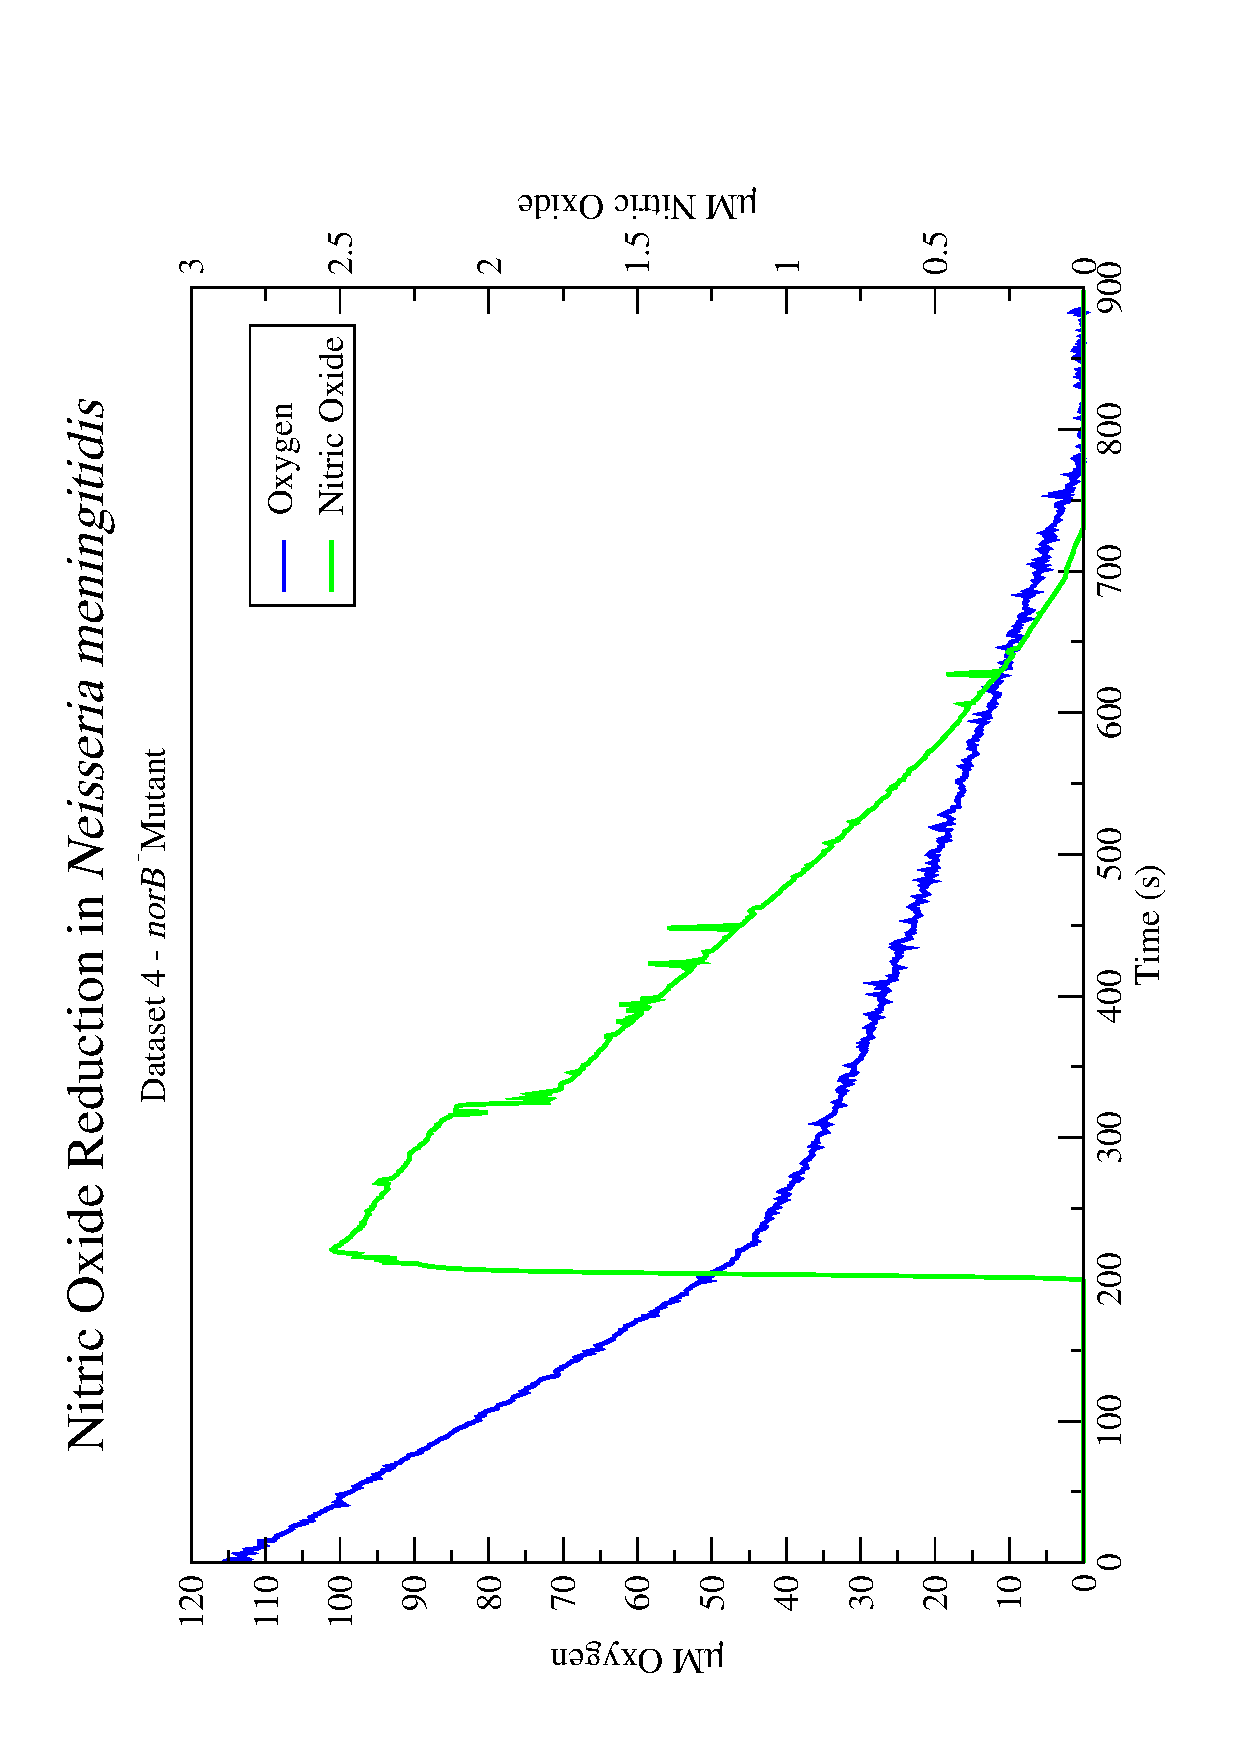
\includegraphics[height=10cm, trim=1cm 1cm 3cm 1cm, clip=true]{./06-noreduction/data/aer-no-data3.pdf}
 % nosim.eps: 0x0 pixel, 300dpi, 0.00x0.00 cm, bb=0 0 794 595
 \caption[{Nitric Oxide Reduction in \textit{Neisseria meningitidis}.}]{{\bf Nitric Oxide Reduction in \textit{Neisseria meningitidis}.} This dataset shows the effect on rate of oxygen reduction as nitric oxide (to $\approx 2.5~\mu M$) is introduced to a respiring $norB-$ mutant culture. Any removal of nitric oxide here is due to diffusion and sequestering by \cbbthree{} alone.}
 \label{fig:nodata3}
\end{figure}
The dataset in Figure \ref{fig:nodata3} shows a visible change in reduction rate of \cbbthree{} upon addition of nitric oxide. This is due to inhibition of the \cbbthree{} directly by nitric oxide. This culture is incapable of reducing nitric oxide, having a $norB^-$ mutation, thus the only route for removal of nitric oxide is by simple diffusion.

\subsubsection{Prior Probability Distributions}
As in Chapter \ref{chap:oxygenreduction} the integrative scheme requires that all the parameters involved have associated prior probability distributions. The posterior probability distributions from Chapter \ref{chap:oxygenreduction} were used as prior probability distributions in this chapter. Where new parameters were introduced (which had not been modelled thus far), the distributions were generated based upon published literature values which are noted in Chapter \ref{chap:model}. When using literature values the prior probability distributions were generated according to the same scheme as in Chapter \ref{chap:oxygenreduction}. Where the posterior probability distributions from Chapter \ref{chap:oxygenreduction} describe rate constants the raw values from the distributions were used as priors in this chapter. Where the distributions describe component concentrations, idealised lognormal distributions were used instead of the raw data to account for differing concentrations between cultures. The distribution of the parameter $\gamma$ - the rate of loss of NO - was initially assumed to be similar to $\beta$, thus the same probability distribution was used. For the other new parameters, lognormal distributions were used as priors as described in Chapter \ref{chap:oxygenreduction}. The values required to create idealised lognormal probability distributions for each parameter are shown in Table \ref{tab:noProbstat1}.

\begin{table}[ht]%needs to be 'here' as section is short
\renewcommand{\arraystretch}{1.5}
\begin{center}
\begin{tabular}{cccc|cccc}
\toprule
\textbf{Parameter} && ${\bar{x}}$ & $\sigma$ & \textbf{Parameter} && ${\bar{x}}$ & $\sigma$\\
\midrule
$k_1$ && 413.228 & 30.046 & g && 0.889 & 0.089\\
$k_3$ && 4.496 & 0.463 & f && 8.707 & 1.35\\
$l_1$ && 6 & 2 & $\gamma$ && 0.00014 & $4.67\times 10^{-6}$\\
$l_3$ && 1 & 2 & Q && 3.143 & 0.240\\
$k_5$ && 100 & 10 & X && 4.732 & 6.707\\
$k_6$ && 38 & 8 & B && 0.043 & 0.044\\
$\beta$ && 0.00014 & $4.67\times 10^{-6}$ & C && 0.043 & 0.044\\
\bottomrule
\end{tabular}
\end{center}
\caption[Prior Probability Table]{{\bf Prior Probability Table} This table shows the prior means and standard deviations used to create lognormal distributions to be used as the prior probability distributions.
\label{tab:noProbstat1}}
\end{table}
\afterpage{\clearpage}
The initial probability distributions used to start the Monte-Carlo runs are shown in Figure \ref{fig:aer_no_priors}.
\begin{figure}[tbp]
 \centering
 \includegraphics[width=15cm, trim=0cm 0cm 0cm 0cm]{./06-noreduction/data/aer-no-priors.pdf}
 % priors.pdf: 1008x1008 pixel, 72dpi, 35.56x35.56 cm, bb=0 0 1008 1008
 \caption[Prior probability distributions for aerobic nitric oxide reduction]{{\bf Prior probability distributions for aerobic nitric oxide reduction}. These are the probability distributions used as priors by the parameter estimation algorithm.
 \label{fig:aer_no_priors}}
\end{figure}
\afterpage{\clearpage}

\subsubsection{Parameter Estimation Results}
The parameter estimation process was run in the same fashion as that described in Chapter \ref{chap:oxygenreduction}. The 3 experimental datasets were run 20 times (each) for 20,000 iterations using the prior probability distributions shown in Figure \ref{fig:aer_no_priors}. This generated parameter trajectories from each of the 3 datasets. The second dataset was still analysed even though it is unlikely that the model will successfully be able to be parametrised from it. Unfortunately upon examination of the \textit{BOF} values from the MHMC output and the best-fitting solved output it was clear that the prior probability distributions in conjunction with the model are incapable of accurately describing the experimental data. This strongly suggested that the new prior probability distributions (those obtained from the literature for the NO related components) were incorrect. The solved output from datasets 1 \& 3 are shown in Figures \ref{fig:nosim1.1} \& \ref{fig:nosim3.1} respectively.

In dataset 1, the reduction of oxygen appears to be being modelled quite accurately. This is due to the largely featureless nature of the reduction curve which can easily be accommodated by the wide prior probability distributions given for the parameters involved. The rate change upon addition of a small amount of nitric oxide is only very slight, thus a perfectly straight line will fit it very well. As can be seen however, nitric oxide removal by diffusion is being modelled very poorly indeed. There is no active NorB in this culture, thus there is no modelled nitric oxide reduction. The prior distribution for the diffusion rate of nitric oxide is clearly incorrect, as nitric oxide removal in the solved output is virtually non-existent.

In dataset 3, reduction of oxygen is being modelled very poorly as the parameters produced by the parameter estimation system do not appear to have captured the behaviour that causes oxygen reduction to cease. In this case the \textit{BOF} value has been minimised by generating a linear reduction of oxygen which doesn't accurately represent either of the observed rates. As has been noted about dataset 1, the rate of nitric oxide diffusion is incorrect, thus in order to obtain a sensible rate for removal/reduction of nitric oxide the rate constants for nitric oxide reduction will have to have been increased artificially. This combination of parameters also means that the reduction in rate of oxygen reduction cannot be modelled correctly. This behaviour should be attributed to temporary chemical inhibition of \cbbthree{} by nitric oxide itself (which is now present in high enough concentrations), and by competition for electrons with NorB.

As in Chapter \ref{chap:oxygenreduction}, the prior probability distributions were incapable of producing parameter sets which accurately model the experimental data, thus making the posterior probability distributions generated invalid. The prior probability distributions were therefore altered in an attempt to improve fitting. In addition to altered prior probability distributions a slightly different parameter estimation protocol was employed which is detailed in the next section.

\begin{figure}[tbp]
 \centering
 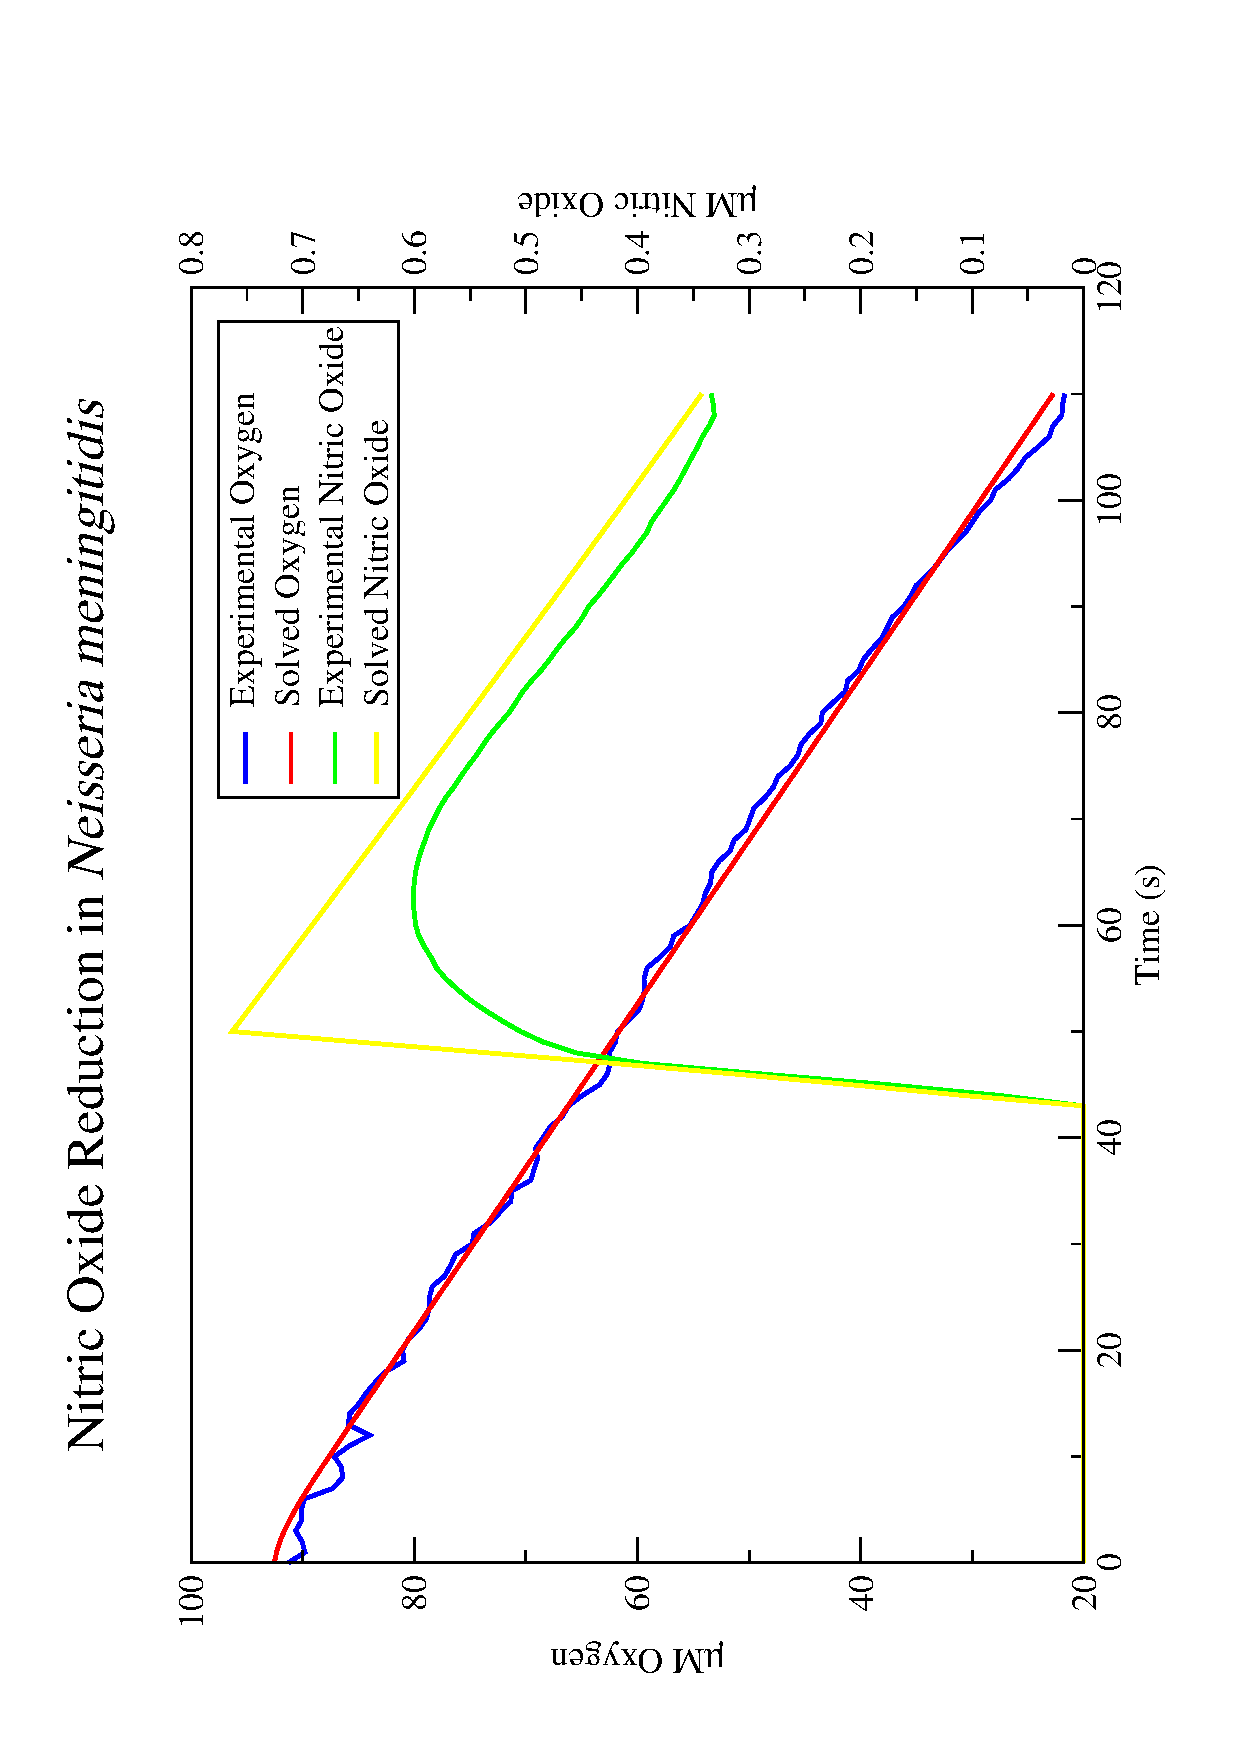
\includegraphics[width=15cm, trim=1cm 1cm 3cm 1cm, clip=true]{./06-noreduction/data/aer-no-sim1.pdf}
 % nosim.eps: 0x0 pixel, 300dpi, 0.00x0.00 cm, bb=0 0 794 595
 \caption[{Nitric Oxide Reduction in \textit{Neisseria meningitidis}.}]{{\bf Nitric Oxide Reduction in \textit{Neisseria meningitidis}.} This figure shows the first attempt at fitting the model to experimental data using priors determined from literature values. Nitric oxide disappearance is not being modelled at all.}
 \label{fig:nosim1.1}
\end{figure}

\begin{figure}[tbp]
 \centering
 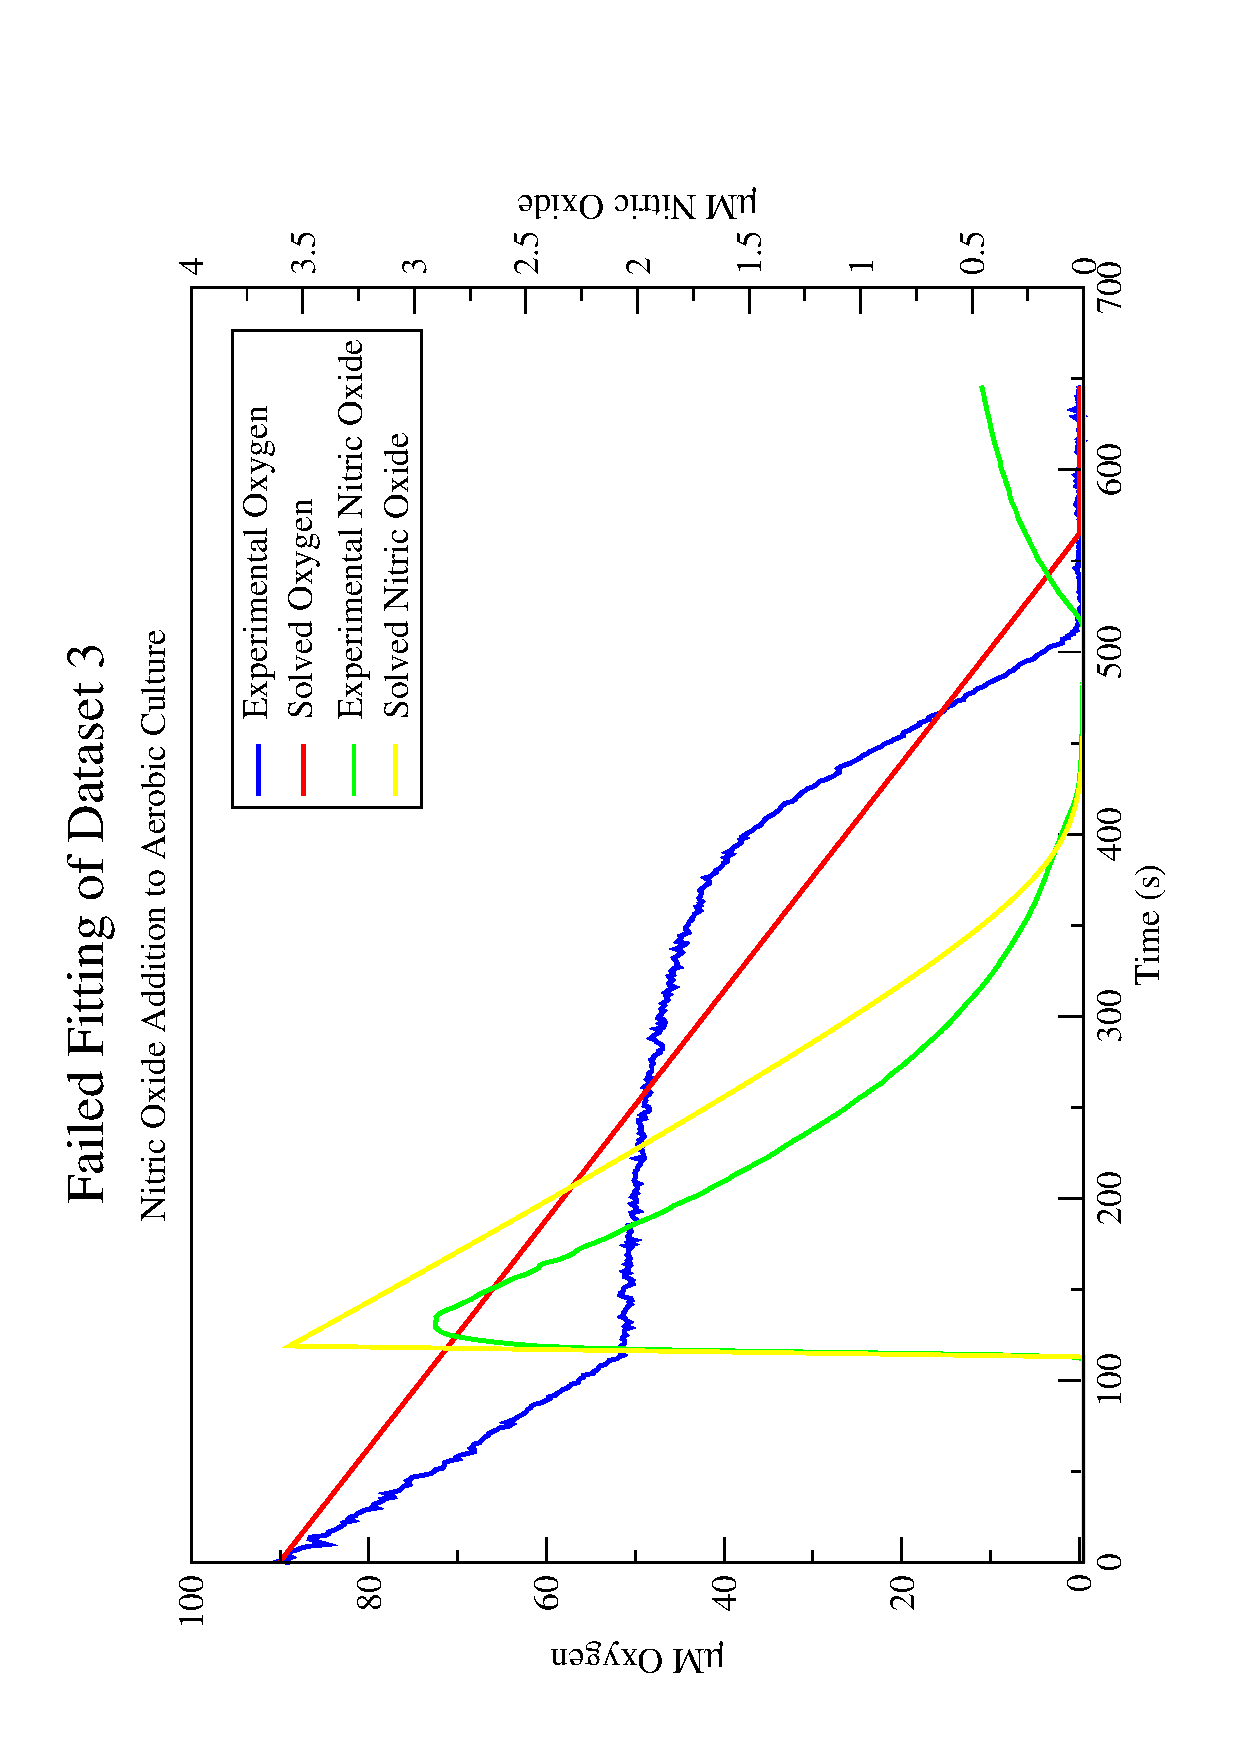
\includegraphics[width=15cm, trim=1cm 1cm 3cm 1cm, clip=true]{./06-noreduction/data/aer-no-sim3.pdf}
 % nosim.eps: 0x0 pixel, 300dpi, 0.00x0.00 cm, bb=0 0 794 595
 \caption[{Nitric Oxide Reduction in \textit{Neisseria meningitidis}.}]{{\bf Nitric Oxide Reduction in \textit{Neisseria meningitidis}.} This figure shows the first attempt at fitting the model to experimental data using priors determined from literature values. Nitric oxide disappearance is now being modelled much more accurately than in Figure \ref{fig:nosim1.1}. Oxygen reduction is not being modelled correctly and the best fitting parameters generate a straight line rather than capturing the stopping and restarting of oxygen reduction.}
 \label{fig:nosim3.1}
\end{figure}

\subsubsection{Adapted Parameter Estimation Protocol}

As dataset 1 was the simplest of the experimental datasets which describe the effects of addition of nitric oxide to aerobically respiring cultures, this dataset could be run as a standalone step in the Bayesian scheme for parameter estimation. This dataset described some of the experimentally observed behaviour in isolation, such as the removal of nitric oxide by diffusion alone, therefore could generate a posterior probability distribution for datasets where that parameter could \textit{not} be examined in isolation. Dataset 3 ideally required this information as a prior probability distribution as the experimentally observed disappearance of nitric oxide was expected to be due to both diffusion and reduction (by NorB). Therefore dataset 1 could be used to inform the prior probability distribution of dataset 3. Statistically this did not pose a problem even though the two datasets were run in parallel previously. This was because the numerical output from those previous attempts was not being used as input for the subsequent attempts.

\subsubsection{Secondary Parameter Estimation Results}
Trial and error was employed to produce an initial informed prior value for $\gamma$, the rate of diffusion of nitric oxide, which was the problematic parameter for dataset 1 previously. This value was estimated to be $\approx 0.02~\mu Ms^{-1}$ based upon visual comparison of the solved output against the experimental data. This value was then used as a prior with no bounds so that the parameter estimation algorithm could home in on the correct distribution. All the other prior probability distributions were left unchanged from the first attempt.

Figure \ref{fig:nosim1.2} shows greatly improved fitting of solved data to experimental values suggesting that the parameters are now correct (or at least reasonably close) for describing the removal of nitric oxide. The model is still not capturing the small effect on oxygen reduction rate visible in the experimental data however. A linear regression of the solved oxygen data suggests that it is in fact a perfectly straight line ($R^2=0.9999$, source data not shown) whereas there should be a slight elbow upon addition of nitric oxide. This was not considered to be a significant problem here, as the effect is far more visible in the subsequent dataset(s), therefore would be more easily modelled.

The posterior probability distributions that this dataset produced after parameter estimation are shown in Figure \ref{fig:dataset1posterior1}. These distributions can be used as prior probability distributions for parameter estimation of dataset 3, as these now include the missing information about rate of removal of nitric oxide by diffusion.

\begin{figure}[tbp]
 \centering
 \includegraphics[width=15cm, trim=1cm 1cm 3cm 1cm, clip=true]{./06-noreduction/data/aer-no-sim1-2.pdf}
 % nosim.eps: 0x0 pixel, 300dpi, 0.00x0.00 cm, bb=0 0 794 595
 \caption[{Nitric Oxide Reduction in \textit{Neisseria meningitidis}.}]{{\bf Nitric Oxide Reduction in \textit{Neisseria meningitidis}.} This figure shows the second attempt at fitting the model to experimental data using priors determined from literature values in addition to manually adjusted priors. Oxygen reduction is modelled almost perfectly, and the shape of the nitric oxide reduction curve is captured well also.}
 \label{fig:nosim1.2}
\end{figure}

\begin{figure}[p]
 \centering
 \includegraphics[width=15cm, trim=0cm 0cm 0cm 0cm]{./06-noreduction/data/posteriors-1.pdf}
 % priors.pdf: 1008x1008 pixel, 72dpi, 35.56x35.56 cm, bb=0 0 1008 1008
 \caption[Posterior Distributions for Dataset 1]{{\bf Posterior Distributions for Dataset 1}. The posterior probability distributions for dataset 1 of nitric oxide removal. All the parameters are still well within their prior bounds with the exception of $\gamma$ which had a manually altered starting value which was significantly different from the original prior distribution. The initial reduced state posteriors appear as point values as the perturbation kernel was disabled for these values (starting value is largely irrelevant).
 \label{fig:dataset1posterior1}}
\end{figure}

\subsubsection{Tertiary Parameter Estimation Results}
The third round of parameter estimation built upon the results from the previous section. After parametrising the value for $\gamma$ from dataset 1, it was then possible to attempt parameter estimation on dataset 3 which also involved $l_1$, $l_3$, $k_5$ \& $k_6$ for reduction of nitric oxide and inactivation of \cbbthree{} by nitric oxide respectively. The prior probability distributions used for this round of parameter estimation were the same as in Figure \ref{fig:aer_no_priors} except that the distribution for $\gamma$ was replaced by that found in Figure \ref{fig:dataset1posterior1}. Additionally the distributions for $k_1$ and $k_3$ were replaced by idealised lognormal distributions to remove the inherent bimodality and hard limits found in those source distributions.

Preliminary test runs (data not shown) using these prior probability distributions suggested that at least one of the two parameters relating to the inactivation of \cbbthree{} by nitric oxide was incorrect for this model. In order to obtain a oxygen reduction curve that matches the general shape of the experimentally obtained data a ratio of $k_5:k_6 \approx 10,000:1$ was required. Since it was unknown which of the two values was more incorrect, both parameters were allowed to be perturbed freely during parameter estimation, i.e. they had no prior probability distribution. Unfortunately this seemed to be the only sensible approach to take given the lack of further data. These preliminary runs suggested that the number of parameter estimation iterations would need to be increased for this dataset also due to the presence of local \textit{BOF} value minima caused by the model fitting oxygen as a straight line between the fixed starting point and the point at which oxygen is depleted similar to the result shown in Figure \ref{fig:nosim3.1}. Figure \ref{fig:nosim3-bof} illustrates local minima phenomenon. Given that this figure shows that a suitably low \textit{BOF} value is not achieved until at least 15000 iterations (and in some cases this extended up to 50000 iterations) a value of 100000 iterations was chosen to ensure that a significant number of data-points were available to generate posterior probability distributions.

\begin{figure}[tbp]
 \centering
 \includegraphics[width=15cm, trim=1cm 1cm 3cm 1cm, clip=true]{./06-noreduction/data/ds3-bof.pdf}
 % nosim.eps: 0x0 pixel, 300dpi, 0.00x0.00 cm, bb=0 0 794 595
 \caption[{Local Fitness Minima During Parameter Estimation.}]{{\bf Local Fitness Minima During Parameter Estimation.} This figure shows the \textit{BOF} value as the MHMC progresses on dataset 3. A local fitness minima is clearly visible at a \textit{BOF} value of approximately 7000 where the parameter estimation algorithm has settled on a straight line for oxygen reduction. After a variable number of iterations the MHMC run exits the local fitness minima and progresses towards a much better fitting set of parameters. This is a typical plot of the \textit{BOF} values, however in some runs the fitness minima is exited much more abruptly rather than the gradual change seen here.}
 \label{fig:nosim3-bof}
\end{figure}

A representative plot showing the solved data after running the parameter estimation system as described above is shown in Figure \ref{fig:nosim3.2}. The model appeared to be able to capture all the features of the oxygen reduction curve including the halting of oxygen reduction upon addition of nitric oxide, and the recovery after nitric oxide has been removed. Similarly to the results seen in Chapter \ref{chap:oxygenreduction} the high degree of \cbbthree{} for oxygen is also captured (probably a little too high). Nitric oxide was generally modelled less well than was hoped. The point of nitric oxide depletion appeared to be modelled correctly, but the rate of reduction of nitric oxide starts too fast and slows too quickly resulting in more pronounced curvature than the experimental data shows.

The concentration of nitric oxide present will also affect the rate of \cbbthree{} reduction (due to the effect of temporary inactivation by nitric oxide), thus implying that the rate constants obtained to describe that effect may not be completely correct. Some of the observed discrepancy between the experimental and solved nitric oxide concentrations may in fact be due to errors introduced into the experimental data by the experimental set up. The nitric oxide electrode was not capable of detecting large changes in concentration quickly and this always resulted in a lag between nitric oxide addition and detection by the electrode. This is obvious in the experimental datasets where the total nitric oxide addition is not captured as the cultures have already started to remove it. This requires backwards extrapolation of the experimental data to determine what the actual added concentration was (and what should be added \textit{in silico} to the model).

\begin{figure}[tbp]
 \centering
 \includegraphics[width=15cm, trim=1cm 1cm 3cm 1cm, clip=true]{./06-noreduction/data/aer-no-sim3-1.pdf}
 % nosim.eps: 0x0 pixel, 300dpi, 0.00x0.00 cm, bb=0 0 794 595
 \caption[{Nitric Oxide Reduction in \textit{Neisseria meningitidis}.}]{{\bf Nitric Oxide Reduction in \textit{Neisseria meningitidis}.} This figure shows the third attempt at fitting the model to experimental data using priors determined from literature values in addition to manually adjusted priors. Oxygen reduction is being modeled remarkably well, whereas the rate of nitric oxide reduction appears to be too high in the solved output.}
 \label{fig:nosim3.2}
\end{figure}

The posterior probability distributions generated from this third round of parameter estimation are shown in Figure \ref{fig:dataset3posterior1}. The distributions generated for the parameters relating solely to oxygen reduction were broadly similar to the prior probability distributions which was to be expected and confirms that these distributions capable of describing the oxygen reduction behaviour. The rate of NO reduction by NorB appeared to be very similar to the prior probability distribution however the rate of NorB reduction seemed to have been vastly overestimated in the prior distribution. The prior distribution for this parameter was unknown however, and was set to a very wide lognormal with mean of 1. The rate of NO diffusion ($\gamma$) tended to settle at the lower end of the prior distribution. The most interesting posterior probability distributions were those of $k_5$ and $k_6$ which actually had to be freely perturbed, rather than be constrained by their prior probability distributions. Neither of these two parameters settled anywhere near the prior probability distributions. Further processing on these data revealed that the ratio between the two values was always between $\approx 10000$ and $\approx 20000$. $k_5$ never settles on a value less than $\approx 1800~\mu M^{-1}s^{-1}$. This value turned out to be a critical threshold to at which the inactivation of \cbbthree{} occurs. At lower values of $k_5$ the inactivation is slower than observed in the experimental dataset and the in the solved data the ``elbow'' is shifted visibly to the right. At or above this threshold the inactivation point closely matches that seen in the experimental dataset. It appeared that that absolute values of $k_5$ and $k_6$ are unimportant, only that $k_5$ is greater than $\approx 1800~\mu M^{-1}s^{-1}$ and that the ratio of $k_5:k_6 \approx 10000:1$ to $20000:1$. Unfortunately this meant that it was impossible to determine if the obtained posterior probability distributions were actually representative of the true distributions.

\begin{figure}[p]
 \centering
 \includegraphics[width=15cm, trim=0cm 0cm 0cm 0cm]{./06-noreduction/data/posteriors-2.pdf}
 % priors.pdf: 1008x1008 pixel, 72dpi, 35.56x35.56 cm, bb=0 0 1008 1008
 \caption[Posterior Distributions for Dataset 3]{{\bf Posterior Distributions for Dataset 3}. The posterior probability distributions for dataset 3 of nitric oxide removal. The initial reduced state posteriors appear as point values as the perturbation kernel was disabled for these values (starting value is largely irrelevant).
 \label{fig:dataset3posterior1}}
\end{figure}

A comparison between the prior and posterior distributions can be seen in tabular form in Table \ref{tab:noPstat}. This table shows the parameters of the idealised lognormal distributions which describe the obtained probability distributions to more easily represent the data.

\begin{table}[tbp]%needs to be 'here' as section is short
\renewcommand{\arraystretch}{1.5}
\begin{center}
\begin{tabular}{cccccc}
\toprule
& & \multicolumn{2}{c}{\textbf{Priors}} & \multicolumn{2}{c}{\textbf{Posteriors}} \\
\textbf{Parameter} && ${\bar{x}}$ & $\sigma$ & ${\bar{x}}$ & $\sigma$\\
\midrule
$k_1$ && 450 & 35 & 395.75$\downarrow$ & 56.36$\downarrow$\\
$k_3$ && 4.748 & 0.404 & 5.44 & 0.65\\
$l_1$ && 6 & 2 & 2.35$\downarrow$ & 1.47$\downarrow$\\
$l_3$ && 1 & 2 & 0.035$\downarrow$ & 0.1$\downarrow$\\
$k_5$ && 100 & 10 & 4170.95$\uparrow$ & 1756.5$\uparrow$\\
$k_6$ && 38 & 8 & 0.3$\downarrow$ & 0.17$\downarrow$\\
$\beta$ && 0.00014 & $4.72\times 10^{-6}$ & 0.00014 & $4.9\times 10^{-6}$\\
g && 1.053 & 0.099 & 1.072 & 0.1\\
f && 9.10 & 1.18 & 8.60 & 2.36$\uparrow$\\
$\gamma$ && 0.00014 & $4.72\times 10^{-6}$ & 0.017$\uparrow$ & 0.0015$\uparrow$\\
Q && 3.59 & 0.132 & 4.20 & 0.70\\
X && 15.177 & 0.247 & 14.52 & 1.25\\
B && 0.143 & 0.159 & 0.23 & 0.03\\
C && 0.143 & 0.159 & 0.06 & 0.01\\
\bottomrule
\end{tabular}
\end{center}
\caption[Posterior Probability Statistics]{{\bf Posterior Probability Statistics.} This table shows the parameters required to create lognormal distributions that describe the prior and posterior probability distributions. The values for the priors are as in Table \ref{tab:noProbstat1}. The posterior distributions were generated from dataset 3 (after being run on dataset 1), and where they relate to concentrations, these have been normalised. The lognormal distributions represent best-fits to the actual posterior distributions. Where there are significant differences between the prior and posterior values for either the mean or standard deviation, these are indicated by $\uparrow$ and $\downarrow$.
\label{tab:noPstat}}
\end{table}

\subsubsection{Analysis of Convergence}
The Gelman-Rubin R statistics were calculated for the Monte-Carlo trajectories for each parameter and these are presented in Table \ref{tab:noRstat}. The newly included parameters all had large R statistic values suggesting that there is still opportunity for scale reduction in the trajectories. This is highly likely to be due to the fact that $k_5$ and $k_6$ had to be unconstrained by prior probability distributions, and they are directly affecting the values of $l_1$ and $l_3$ in such a way as to prevent them converging fully. Some of the oxygen reduction parameters actually had slightly larger R statistic values than the results from Chapter \ref{chap:oxygenreduction}.

\begin{table}[tbp]%needs to be 'here' as section is short
\renewcommand{\arraystretch}{1.5}
\begin{center}
\begin{tabular}{ccc|ccc}
\toprule
\textbf{Parameter} && \textbf{R value} & \textbf{Parameter} && \textbf{R value}\\
\midrule
$k_1$ && 1.27 & g && 3.50\\
$k_3$ && 3.87 & f && 4.78\\
$l_1$ && 11.86 & $\gamma$ && 1.66\\
$l_3$ && 4.44 & Q && 3.15\\
$k_5$ && 15.74 & X && 2.76\\
$k_6$ && 13.13 & B && 3.44\\
$\beta$ && 1.36 & C && 4.04 \\
\bottomrule
\end{tabular}
\end{center}
\caption[Gelman-Rubin Convergence Statistic]{{\bf Gelman-Rubin Convergence Statistic.} This table shows the Gelman-Rubin Convergence statistic for all the Markov chains from dataset 3. For parameters which are concentrations, the statistic relates to the values after normalisation (data is normalised based on initial oxygen reduction rate).
\label{tab:noRstat}}
\end{table}

\subsubsection{Analysis of Correlation}
A correlation analysis was performed on each of the parameters using the Monte-Carlo trajectories as in Chapter \ref{chap:oxygenreduction}. The upper-triangle correlation matrix is shown in Table \ref{tab:noregress1}. The correlation matrix shows a much greater degree of correlation between parameter values than was seen in for oxygen reduction alone. There were much stronger correlations between C and $k_3$ and C and X for this dataset than for oxygen reduction, but the direction of correlation was the same which made sense. Additionally there was a very strong positive correlation between $k_5$ and $k_6$, which given the brief discussion earlier in the chapter was to be expected. As it appeared that the ratio and not the absolute values of $k_5$ and $k_6$ was important, a strong positive correlation between values would achieve this.

There were a number of other interesting correlation between parameters also. $l_3$ - the rate of reduction of NorB appeared to be strongly negatively correlated to $\gamma$- the rate of NO loss. This could be explained by the model needing to balance the removal of NO by simple diffusion and by reduction. Increasing the rate of diffusion could be offset by decreasing the rate of reduction of NorB which in turn would slow down NO reduction. There also appeared to be a strong negative correlation between the amount of quinones, Q, and $l_3$, which would make sense if the model were trying to maintain a constant level of NorB reduction. More quinones would lead to a slower rate of reduction being required to maintain the same level of reduction. This same negative correlation can also be observed between Q and $k_3$ \& C to achieve the same result for reduction state of \cbbthree{}.The positions in the electron transport chain of these correlations are shown below, marked by superscript $\blacktriangle$, $\square$, $\bigstar$, $\Diamond$ and $\clubsuit$.
\begin{equation*}
\xrightarrow{g}Q^\clubsuit\xrightarrow{f}X^{\blacktriangle}\xrightarrow{k_3^{\square}}C^{\square\blacktriangle}\xrightarrow{k_1}O_2
\end{equation*}
\begin{equation*}
NO + C_a \mathop{\leftrightharpoons}_{k_6^{\bigstar}}^{k_5^{\bigstar}}NO\mhyphen C_X
\end{equation*}
\begin{equation*}
\xrightarrow{g}Q^\clubsuit\xrightarrow{l_1}B\xrightarrow{l_3^{\Diamond\clubsuit}} NO
\end{equation*}
\begin{equation*}
NO\xrightarrow{\gamma^\lozenge}\emptyset
\end{equation*}



\begin{table}[p]
\setlength{\tabcolsep}{5pt}
\renewcommand{\arraystretch}{1.5}
  \centering
  \rotatebox{90}{
  \begin{minipage}{24.4cm}
  \centering
  \begin{tabular}{|c|c|c|c|c|c|c|c|c|c|c|c|c|c|c|}
    \hline
    \cellcolor{dark-gray} & \cellcolor{dark-gray}$k_1$ & \cellcolor{dark-gray}$k_3$ & \cellcolor{dark-gray}$l_1$ & \cellcolor{dark-gray}$l_3$ & \cellcolor{dark-gray}$k_5$ & \cellcolor{dark-gray}$k_6$ & \cellcolor{dark-gray}$\beta$ & \cellcolor{dark-gray}g & \cellcolor{dark-gray}f & \cellcolor{dark-gray}$\gamma$ & \cellcolor{dark-gray}Q & \cellcolor{dark-gray}X & \cellcolor{dark-gray}B & \cellcolor{dark-gray}C \\
    \hline
    \cellcolor{dark-gray}$k_1$ & \cellcolor{light-gray}1 & -0.05 & 0.03 & 0.06 & -0.02 & -0.06 & -0.02 & 0.01 & -0.05 & -0.05 & -0.10 & -0.11 & 0.02 & 0.08 \\
    \hline
    \cellcolor{dark-gray}$k_3$ & \cellcolor{light-gray} & \cellcolor{light-gray}1 & \cellcolor{orange}-0.53 & \cellcolor{orange}-0.45 & 0.16 & 0.27 & 0.0022 & -0.08 & 0.15 & \cellcolor{orange}0.48 & \cellcolor{orange}0.57 & \cellcolor{orange}0.55 & 0.18 & \cellcolor{green}-0.91 \\
    \hline
    \cellcolor{dark-gray}$l_1$ & \cellcolor{light-gray} & \cellcolor{light-gray} & \cellcolor{light-gray}1 & 0.18 & -0.07 & -0.15 & -0.008 & 0.15 & -0.05 & -0.14 & \cellcolor{orange}-0.34 & \cellcolor{orange}-0.50 & \cellcolor{orange}-0.49 & \cellcolor{orange}0.58\\
    \hline
    \cellcolor{dark-gray}$l_3$ & \cellcolor{light-gray} & \cellcolor{light-gray} & \cellcolor{light-gray} & \cellcolor{light-gray}1 & -0.10 & -0.05 & -0.02 & 0.003 & \cellcolor{orange}-0.20 & \cellcolor{orange}-0.70 & \cellcolor{orange}-0.69 & \cellcolor{orange}-0.44 & \cellcolor{orange}-0.32 & \cellcolor{orange}0.53\\
    \hline
    \cellcolor{dark-gray}$k_5$ & \cellcolor{light-gray} & \cellcolor{light-gray} & \cellcolor{light-gray} & \cellcolor{light-gray} & \cellcolor{light-gray}1 & \cellcolor{green}0.93 & 0.10 & -0.03 & -0.19 & -0.03 & 0.03 & 0.11 & -0.16 & -0.16\\
    \hline
    \cellcolor{dark-gray}$k_6$ & \cellcolor{light-gray} & \cellcolor{light-gray} & \cellcolor{light-gray} & \cellcolor{light-gray} & \cellcolor{light-gray} & \cellcolor{light-gray}1 & 0.11 & 0.02 & -0.12 & -0.14 & 0.09 & 0.26 & -0.12 & \cellcolor{orange}-0.30\\
    \hline
    \cellcolor{dark-gray}$\beta$ & \cellcolor{light-gray} & \cellcolor{light-gray} & \cellcolor{light-gray} & \cellcolor{light-gray} & \cellcolor{light-gray} & \cellcolor{light-gray} & \cellcolor{light-gray}1 & 0.007 & -0.06 & 0.03 & -0.02 & 0.02 & -0.002 & -0.01 \\
    \hline
    \cellcolor{dark-gray}g & \cellcolor{light-gray} & \cellcolor{light-gray} & \cellcolor{light-gray} & \cellcolor{light-gray} & \cellcolor{light-gray} & \cellcolor{light-gray} & \cellcolor{light-gray} & \cellcolor{light-gray}1 & -0.07 & -0.01 & -0.01 & 0.10 & -0.10 & -0.02 \\
    \hline
    \cellcolor{dark-gray}f & \cellcolor{light-gray} & \cellcolor{light-gray} & \cellcolor{light-gray} & \cellcolor{light-gray} & \cellcolor{light-gray} & \cellcolor{light-gray} & \cellcolor{light-gray} & \cellcolor{light-gray} & \cellcolor{light-gray}1 & 0.27 & 0.21 & 0.11 & 0.05 & -0.17\\
    \hline
    \cellcolor{dark-gray}$\gamma$ & \cellcolor{light-gray} & \cellcolor{light-gray} & \cellcolor{light-gray} & \cellcolor{light-gray} & \cellcolor{light-gray} & \cellcolor{light-gray} & \cellcolor{light-gray} & \cellcolor{light-gray} & \cellcolor{light-gray} & \cellcolor{light-gray}1 & \cellcolor{orange}0.50 & \cellcolor{orange}0.40 & -0.02 & \cellcolor{orange}-0.48\\
    \hline
    \cellcolor{dark-gray}Q & \cellcolor{light-gray} & \cellcolor{light-gray} & \cellcolor{light-gray} & \cellcolor{light-gray} & \cellcolor{light-gray} & \cellcolor{light-gray} & \cellcolor{light-gray} & \cellcolor{light-gray} & \cellcolor{light-gray} & \cellcolor{light-gray} & \cellcolor{light-gray}1 & \cellcolor{orange}0.63 & -0.03 & \cellcolor{orange}-0.68\\
    \hline
    \cellcolor{dark-gray}X & \cellcolor{light-gray} & \cellcolor{light-gray} & \cellcolor{light-gray} & \cellcolor{light-gray} & \cellcolor{light-gray} & \cellcolor{light-gray} & \cellcolor{light-gray} & \cellcolor{light-gray} & \cellcolor{light-gray} & \cellcolor{light-gray} & \cellcolor{light-gray} & \cellcolor{light-gray}1 & 0.14 & \cellcolor{green}-0.81 \\
    \hline
    \cellcolor{dark-gray}B & \cellcolor{light-gray} & \cellcolor{light-gray} & \cellcolor{light-gray} & \cellcolor{light-gray} & \cellcolor{light-gray} & \cellcolor{light-gray} & \cellcolor{light-gray} & \cellcolor{light-gray} & \cellcolor{light-gray} & \cellcolor{light-gray} & \cellcolor{light-gray} & \cellcolor{light-gray} & \cellcolor{light-gray}1 & -0.20\\
    \hline
    \cellcolor{dark-gray}C & \cellcolor{light-gray} & \cellcolor{light-gray} & \cellcolor{light-gray} & \cellcolor{light-gray} & \cellcolor{light-gray} & \cellcolor{light-gray} & \cellcolor{light-gray} & \cellcolor{light-gray} & \cellcolor{light-gray} & \cellcolor{light-gray} & \cellcolor{light-gray} & \cellcolor{light-gray} & \cellcolor{light-gray} & \cellcolor{light-gray}1\\
    \hline
  \end{tabular}
  \caption[Regression Analysis of Nitric Oxide Reduction Parameters]{{\bf Regression Analysis of Nitric Oxide Reduction Parameters for Dataset 3.} This table shows the $R$ values from linear regression analysis on the parameter trajectories for nitric oxide reduction. Parameters with high correlation have been coloured green ($R\geq0.8$) and those with moderation correlation have been coloured orange ($0.8>R\geq0.3$).
  \label{tab:noregress1}}
  \end{minipage}
  }
\end{table}
\afterpage{\clearpage}
%\end{landscape}
\subsection{Discussion}
The parameter distributions obtained from this more convoluted set of datasets are capable of modelling the experimental data impressively well given the lack of prior information available and taking into account the assumptions made about the system. Oxygen reduction can be modelled almost perfectly using posterior distributions from earlier datasets which will still fit new data. Nitric oxide reduction and removal was modelled less well, however it was not clear whether this was due to a limitation of the model itself, or and inherent issue with the experimental set-up. In reality it was probably a combination of both which would be impossible to decouple. The general features of nitric oxide reduction were captured in the model even if a precise fit wasn't achieved. There were a large number of unknowns in these experimental datasets, it was not clear for example how much NorB was present in dataset 3, therefore the concentrations and rates obtained will most likely not reflect \textit{in vivo} values, however they do provide valuable information about how they interact with other parameters. It is possible that the difference in observed and solved nitric oxide reduction rates is actually due in part to an overestimation of $\gamma$ introduced by the analysis of the first dataset in Figure \ref{fig:nodata1}. It was assumed that there was no NorB present in that culture, thus any and all nitric oxide removal would solely be due to diffusion. If this were \textit{not} the case, and in fact there was some small amount of nitric oxide reductase activity, then $\gamma$ would be overestimated as it would include this NorB activity. The posterior probability distributions for dataset 3 (Figure \ref{fig:dataset3posterior1}) potentially support this hypothesis as they should the parameter estimation system trying to reduce the value of $\gamma$ to the lower limit of its range. This inappropriately high value of $\gamma$ could account for much of the discrepancy between the reduction rates of the experimental and solved data.

The simulated results and parameter set generated from parameter estimation are corroborated by experimental data observed by \citet{Anjum2002}. Small concentrations of NO added result in no visible change in oxygen reduction rate (Figure 5a). Larger concentrations of NO appear to slow the rate of oxygen reduction which is then recovered (Figure 5b). A NorB mutant treated to a larger concentration of NO shows a much slower recovery of oxygen (Figure 5c) which can be shown \textit{in silico} simply be removing NorB.

As more parameters had been populated in the model it was now possible to examine the reduction states of the various enzymes in the system as respiration progresses. A plot showing these states can be seen in Figure \ref{fig:nosimredox}. This figure shows that the reduction states of the enzymes are quickly adjusted to the correct steady state values (of the order of a few seconds) except for NorB, which seems to have a much slower rate of reduction. This slow rate of reduction means that the initial concentration of reduced NorB in the simulation is much more important, and should in fact be much closer to being in a completely reduced state at $t_0$. The virtually instantaneous oxidation of NorB suggests that NorB is very good at reducing nitric oxide. The cytochrome pool appears to stay almost fully reduced throughout the entire simulation, as the rate of cytochrome reduction significantly outweighs the rate of oxidation by downstream components. The quinone pool starts at roughly 70\% reduced, a value which matches what has been observed experimentally. The high rate of \cbbthree{} inactivation also means that upon addition of nitric oxide, 90\% of \cbbthree{} becomes inactivated instantaneously.

\begin{figure}[tbp]
 \centering
 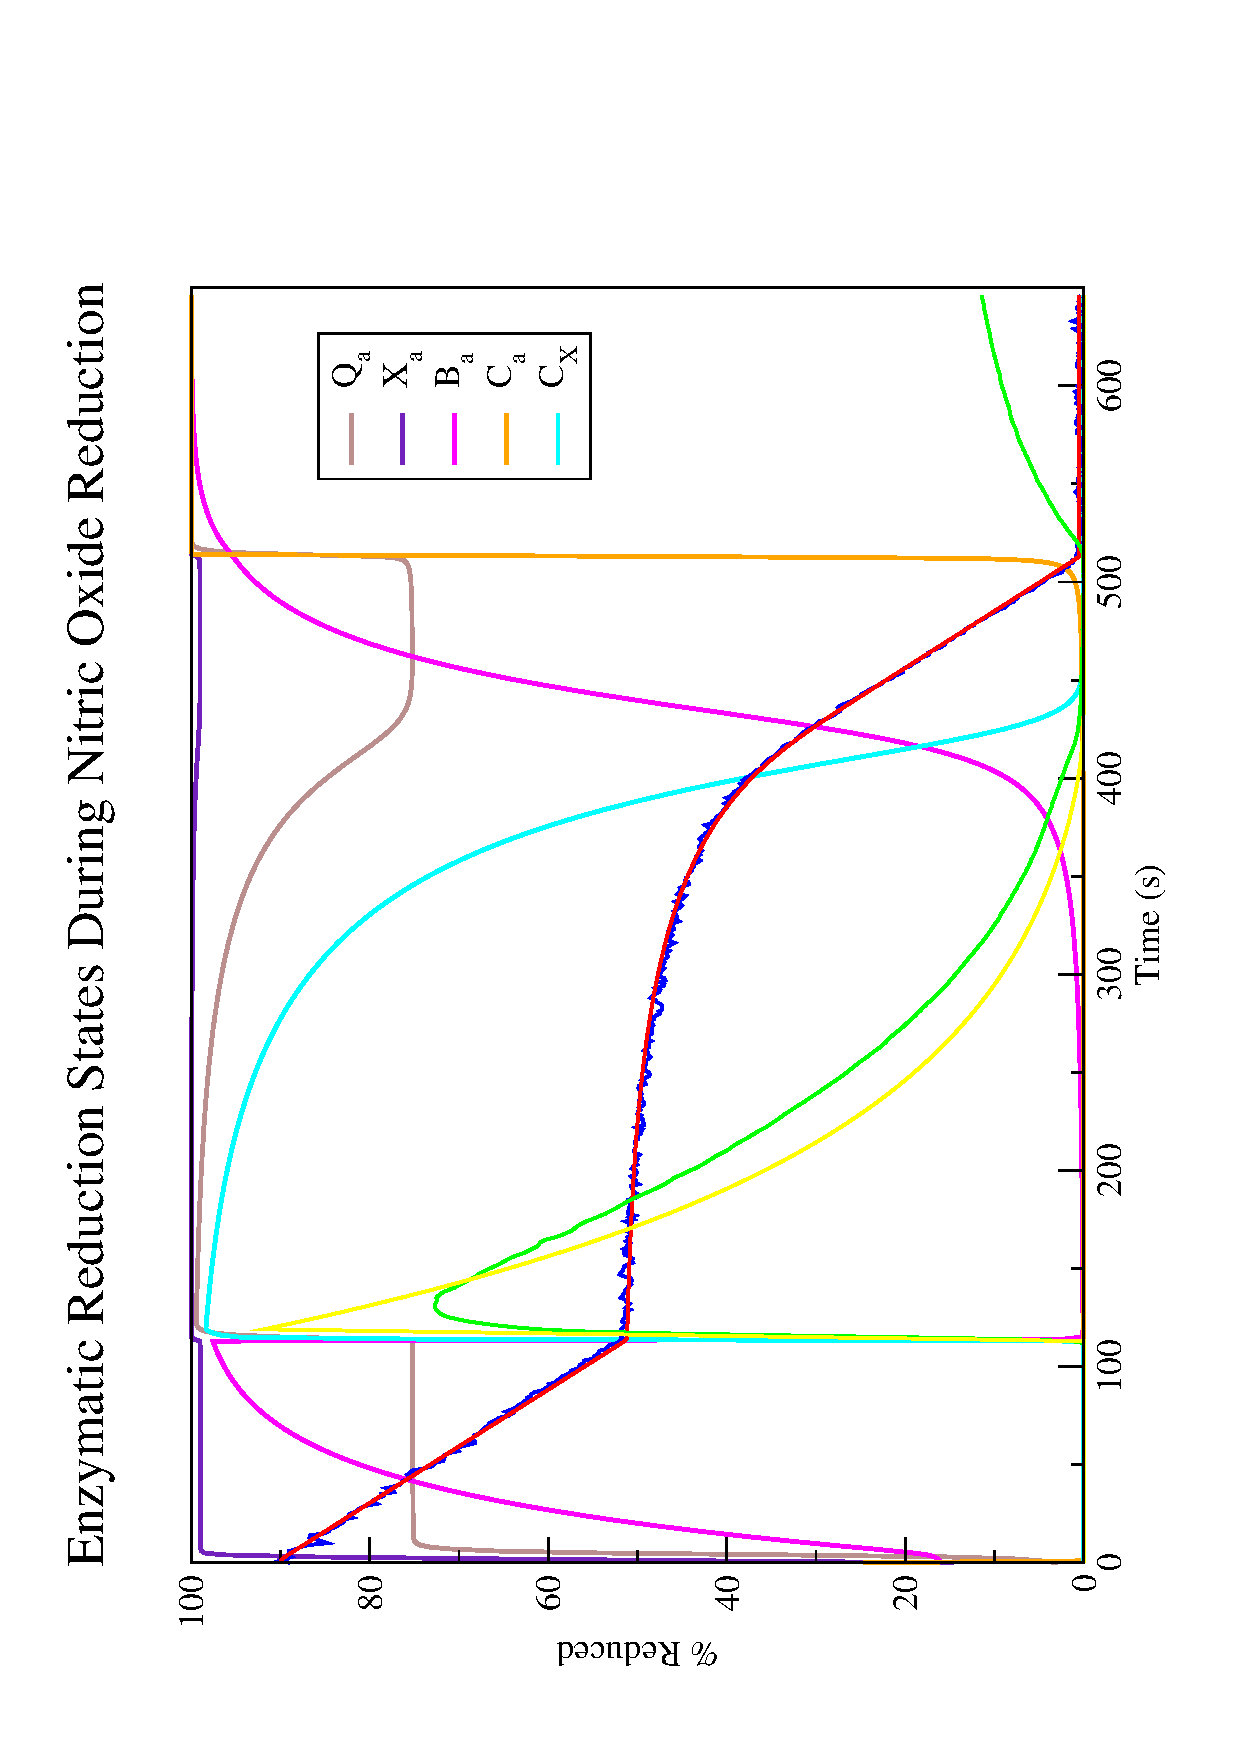
\includegraphics[width=15cm, trim=1cm 1cm 3cm 1cm, clip=true]{./06-noreduction/data/aer-no-sim-redox.pdf}
 % nosim.eps: 0x0 pixel, 300dpi, 0.00x0.00 cm, bb=0 0 794 595
 \caption[{Reduction States During Nitric Oxide Reduction.}]{{\bf Reduction States During Nitric Oxide Reduction.} This figure shows how the reduction states of the enzymes involved in respiration changes as the culture respires oxygen and then nitric oxide. The experimental and solved observed data are shown as dots for reference.}
 \label{fig:nosimredox}
\end{figure}

\section{Redo with correct solver}
\begin{figure}[p]
 \centering
 \includegraphics[width=15cm, trim=0cm 0cm 0cm 0cm]{./06-noreduction/data/posteriors-redo2.pdf}
 % priors.pdf: 1008x1008 pixel, 72dpi, 35.56x35.56 cm, bb=0 0 1008 1008
 \caption[Posterior Distributions for Datasets 1 and 4]{{\bf Posterior Distributions for Datasets 1 and 4}. The posterior probability distributions for datasets 1 and 4 of nitric oxide removal.
 \label{fig:redoneposterior2}}
\end{figure}

\begin{table}[tbp]%needs to be 'here' as section is short
\renewcommand{\arraystretch}{1.5}
\begin{center}
\begin{tabular}{cccccc}
\toprule
& & \multicolumn{2}{c}{\textbf{Priors}} & \multicolumn{2}{c}{\textbf{Posteriors}} \\
\textbf{Parameter} && ${\bar{x}}$ & $\sigma$ & ${\bar{x}}$ & $\sigma$\\
\midrule
$k_1$ && 413.228 & 30.046 & 417.88 & 31.172\\
$k_3$ && 4.496 & 0.463 & 4.65 & 0.619\\
$l_1$ && 6 & 2 & 13.12$\uparrow$ & 8.321$\uparrow$\\
$l_3$ && 1 & 2 & 0.058$\downarrow$ & 0.021$\downarrow$\\
$k_5$ && 100 & 10 & 1741.8$\uparrow$ & 1822.0$\uparrow$\\
$k_6$ && 38 & 8 & 1.076$\downarrow$ & 1.473$\downarrow$\\
$\beta$ && 0.00014 & $4.72\times 10^{-6}$ & 0.00014 & $4.7\times 10^{-6}$\\
g && 0.889 & 0.089 & 0.857 & 0.086\\
f && 8.707 & 1.35 & 8.398 & 1.237\\
$\gamma$ && 0.00014 & $4.72\times 10^{-6}$ & \\
Q && 3.143 & 0.240 & 7.06 & 1.317\\
X && 4.732 & 6.707 & 27.45 & 12.08\\
B && 0.043 & 0.044 & 0.137 & 0.048\\
C && 0.043 & 0.044 & 0.071 & 0.029\\
\bottomrule
\end{tabular}
\end{center}
\caption[Posterior Probability Statistics]{{\bf Posterior Probability Statistics.} This table shows the parameters required to create lognormal distributions that describe the prior and posterior probability distributions. The values for the priors are as in Table \ref{tab:noProbstat1}. The posterior distributions were generated from dataset 3 (after being run on dataset 1), and where they relate to concentrations, these have been normalised. The lognormal distributions represent best-fits to the actual posterior distributions. Where there are significant differences between the prior and posterior values for either the mean or standard deviation, these are indicated by $\uparrow$ and $\downarrow$.
\label{tab:redone-prob-stat}}
\end{table}

\begin{table}[tbp]%needs to be 'here' as section is short
\renewcommand{\arraystretch}{1.5}
\begin{center}
\begin{tabular}{ccc|ccc}
\toprule
\textbf{Parameter} && \textbf{R value} & \textbf{Parameter} && \textbf{R value}\\
\midrule
$k_1$ && 1.15 & g && 1.13\\
$k_3$ && 1.31 & f && 1.20\\
$l_1$ && 4.92 & $\gamma$ && \\
$l_3$ && 131.447 & Q && 1.54\\
$k_5$ && 6.46 & X && 3.82\\
$k_6$ && 7.37 & B && 6.74\\
$\beta$ && 1.02 & C && 2.92 \\
\bottomrule
\end{tabular}
\end{center}
\caption[Gelman-Rubin Convergence Statistic]{{\bf Gelman-Rubin Convergence Statistic.} This table shows the Gelman-Rubin Convergence statistic for all the Markov chains from dataset 3. For parameters which are concentrations, the statistic relates to the values after normalisation (data is normalised based on initial oxygen reduction rate).
\label{tab:noRstat-redone}}
\end{table}

%\section{Microaerobic Nitric Oxide Reduction}
%\subsection{Introduction}
%\subsection{Results}
%\subsection{Discussion}
\section{\texorpdfstring{Aerobic Nitric Oxide Reduction in \textit{nsrR$^\textrm{-}$} mutant}{Aerobic Nitric Oxide Reduction in nsrR- mutant}}
%\subsection{Introduction}
 The $\mathit{nsrR}^-$ mutant, which expresses NorB in an essentially constitutive manner was not effective in generating a usable dataset as it removed any NO almost instantaneously resulting in an almost featureless dataset (data not shown). \textit{Either expand or remove this section}
%\subsection{Results}
%\subsection{Discussion}
\chapter{Nitrite Reduction in \Nm}
\section{Anaerobic Nitrite Reduction}
\subsection{Introduction}
\subsection{Results}
\subsection{Discussion}
\section{Anaerobic Nitrite Reduction in \textit{norB$^\textrm{-}$} mutant}
\subsection{Introduction}
\subsection{Results}
\subsection{Discussion}
\section{Aerobic Nitrite Reduction in \textit{nsrR$^\textrm{-}$} mutant}
\subsection{Introduction}
\subsection{Results}
\subsection{Discussion}
\section{Aerobic Nitrite Reduction in \textit{nsrR$^\textrm{-}$-norB$^\textrm{-}$} mutant}
\subsection{Introduction}
\subsection{Results}
\subsection{Discussion}
\chapter{AniA and NorB expression in \Nm}
\section{Aerobic and Anaerobic Expression}
\subsection{Introduction}
\subsection{Results}
\subsection{Discussion}
\svnid{$Id$}
\chapter{Discussion and Completed Model}
\label{chap:completedmodel}
%Therefore I have integrated microbiological techniques with mathematical modelling principles to allow us to understand the system in a way previously not possible. I have constructed a mathematical model which describes \Nsm{} respiration \textit{in silico} and can produce predictions for the system \textit{in vivo}. To parametrise this model I used a novel integrative scheme where a standard Bayesian fitting methodology is interleaved with iterative experimental data collection on progressively more complex respiratory scenarios.

\section{Amalgamation of cytochromes}

\appendix
\chapter{Appendix}
\begin{eqnarray}
\frac{d[O_2]}{dt} & = & \beta\left(1-\frac{[O_2]}{K_O}\right) - k_{1}[C_a][O_2] \nonumber \\
\frac{d[NO]}{dt} & = & m_{1}[NO_2^-][A_a] - l_1[NO][B_a] - k_5[C_a][NO] + k_6[C_X] - \gamma[NO] \nonumber \\
\frac{d[NO_2^-]}{dt} & = & - m_{1}[NO_2^-][A_a] \nonumber \\
\frac{d[Q_a]}{dt} & = & g([Q] - [Q_a]) - l_3[Q_a]([B] - [B_a]) - f[Q_a]([X]-[E])\ \nonumber \\
\frac{d[E]}{dt} & = & -k_3([C] - [C_a] - [C_X])[E] - m_3([A] - [A_a])[E] + f[Q_a]([X]-[E]) \nonumber \\
\frac{d[A_a]}{dt} & = & m_3([A] - [A_a])[E] - m_{1}[NO_2^-][A_a] \nonumber \\
\frac{d[B_a]}{dt} & = & l_3[Q_a]([B] - [B_a]) - l_1[NO][B_a] \nonumber \\
\frac{d[C_a]}{dt} & = & k_3([C] - [C_a] - [C_X])[E] - k_{1}[C_a][O_2] - k_{5}[C_a][NO] \nonumber \\
\frac{d[C_X]}{dt} & = & k_5[C_a][NO] - k_6 [C_X] \nonumber \\
\frac{d[A]}{dt} & = & \left(R\left(1 - \frac{[O_2] + k_{10}[NO]}{[O_2] + k_{10}[NO] + k_{11}}\right) - S\left(1 - \frac{[NO]}{[NO] + k_{13}}\right)\right) - k_8[A] \nonumber \\
\frac{d[B]}{dt} & = & T \left(\frac{[NO]}{[NO] + k_{15}}\right) - k_{16}[B]
\end{eqnarray}

\begin{table}[ht]
\begin{center}
\caption{Model Variables}
\begin{tabular}{lcc}
\toprule
\textbf{Symbol} & & \textbf{Description}\\
\midrule
$O_2$ & & Oxygen concentration\\
$NO$ & & Nitric oxide concentration\\
$NO_2^-$ & & Nitrite concentration\\
$E$ & & Reduced cytochrome concentration\\
$A_a$& & Reduced AniA\\
$B_a$& & Reduced NorB\\
$C_a$& & Reduced \cbbthree{}\\
$C_X$& & Reversibly inhibited \cbbthree{}\\
$Q_a$& & Reduced Quinones\\
\bottomrule
\end{tabular}
\label{vs}
\end{center}
\end{table}



\begin{table}[ht]
\begin{center}
\caption{Model Parameters}
\begin{tabular}{l c}
\toprule
\textbf{Symbol} & \textbf{Description}\\
\midrule
$k_1$ & Rate of O$_{\textrm{2}}$ reduction by reduced \cbbthree{}\\
$k_3$ & Rate of \cbbthree{} reduction by cytochrome pool\\ 
$l_1$ & Rate of NO reduction by reduced NorB\\
$l_3$ & Rate of NorB reduction by quinone pool\\
$m_1$ & Rate of NO$_{\textrm{2}}^{\textrm{-}}$ reduction by reduced AniA\\
$m_3$ & Rate of AniA reduction by cytochrome pool\\
$k_5$ & Rate of \cbbthree{} inhibition by NO\\
$k_6$ & Rate of recovery of NO inhibited \cbbthree{}\\
$\beta$ & Rate of passive diffusion in of O$_{\textrm{2}}$\\
$K_O$ & Saturation O$_{\textrm{2}}$ level\\
$g$ & Rate of electrons in from NADH\\
$f$ & Rate of reduction of cytochromes by quinones\\
$\gamma$ & Spontaneous loss of NO\\
$Q$ & Concentration of quinones\\
$X$ & Concentration of cytochromes\\   
$A$ & Concentration of AniA\\
$B$ & Concentration of NorB\\
$C$ & Concentration of \cbbthree{}\\
\bottomrule
\end{tabular}
\label{ps}
\end{center}
\end{table}
\backmatter

\newpage

\singlespacing

\printnomenclature[3cm]
\doublespacing

\renewcommand{\bibname}{References}
\addcontentsline{toc}{chapter}{\bibname}

\bibliography{phd_refs}

\end{document}
